% base
\documentclass[oneside]{book}

% characters
\usepackage[T1]{fontenc}
\usepackage[utf8x]{inputenc}

\usepackage{stmaryrd}
\SetSymbolFont{stmry}{bold}{U}{stmry}{m}{n}

\usepackage{comment}

% math
\usepackage{amsmath}
\usepackage{mathtools}

% graphics
\usepackage{mathdots}
\usepackage{nicematrix}
\setcounter{MaxMatrixCols}{20}
\usepackage{rotating}
\definecolor{lblue}{rgb}{.80, .90, .95}
\definecolor{lorange}{rgb}{1, .85, .60}

\usepackage{color}
\definecolor{keywordcolor}{rgb}{0.7, 0.1, 0.1} % red
\definecolor{commentcolor}{rgb}{0.4, 0.4, 0.4} % grey
\definecolor{symbolcolor}{rgb}{0.0, 0.1, 0.6}  % blue
\definecolor{sortcolor}{rgb}{0.1, 0.5, 0.1}    % green

\usepackage{graphicx}

% font
% \usepackage{mathpazo}
% \usepackage{eulervm}
\usepackage{amsfonts}

% code
\usepackage{listings}
\def\lstlanguagefiles{lstlean.tex}
\lstset{language=lean}
\usepackage{float}

% sections
\usepackage{emptypage}
\usepackage{titlesec}
\titleformat{\chapter}{\normalfont\huge\bfseries}{\thechapter.}{20pt}{\huge}

% theorems
\usepackage{amsthm}
\theoremstyle{definition}
\newtheorem{definition}{Definition}
\newtheorem*{definition*}{Definition}

\theoremstyle{remark}
\newtheorem{remark}{Remark}

\theoremstyle{plain}
\newtheorem{proposition}{Proposition}
\newtheorem{theorem}{Theorem}
\newtheorem{claim}{Claim}

% hyphenation
\usepackage{hyphenat}
\hyphenation{pri-mi-tive}

% other
\usepackage[colorlinks=true, linkcolor=teal, urlcolor=blue, citecolor=cyan]{hyperref}
\usepackage{csquotes}

% macro
% \newcommand{\svdots}{\scriptscriptstyle \boldsymbol \vdots}
\newcommand{\perm}[1]{\scriptstyle \left\rmoustache #1 \right\rmoustache}
\newcommand{\bloch}[2]{\Block[draw=white,fill=lblue,line-width=.5mm,rounded-corners]{#1}{#2}} % https://en.wikipedia.org/wiki/Ernest_Bloch
\newcommand{\oloch}[2]{\Block[draw=white,fill=lorange,line-width=.5mm,rounded-corners]{#1}{#2}}
\newcommand{\conv}[1]{\overbracket[.5pt][1pt]{\underbracket[.5pt][1pt]{#1}}}

\newcommand{\NN}{\mathbb{N}}
\newcommand{\ZZ}{\mathbb{Z}}
\newcommand{\RR}{\mathbb{R}}

\newcommand{\floor}[1]{\left\lfloor #1 \right\rfloor}

\newcommand{\gl}{\text{\guillemotleft}}
\newcommand{\gr}{\text{\guillemotright}}

\newcommand{\RPP}{\mathsf{RPP}}
\newcommand{\ORPP}{\mathsf{ORPP}}
\newcommand{\rppf}{\mathsf{f}}
\newcommand{\rppg}{\mathsf{g}}
\newcommand{\rpph}{\mathsf{h}}
\newcommand{\rppId}{\mathsf{Id}}
\newcommand{\rppNe}{\mathsf{Ne}}
\newcommand{\rppSu}{\mathsf{Su}}
\newcommand{\rppPr}{\mathsf{Pr}}
\newcommand{\rppSw}{\mathsf{Sw}}
\newcommand{\rppCo}{\fatsemi}
\newcommand{\rppPa}{\Vert}
\newcommand{\rppIt}{\mathsf{It}}
\newcommand{\rppIta}{\mathsf{Ita}}
\newcommand{\rppItr}{\mathsf{Itr}}
\newcommand{\rppIf}{\mathsf{If}}
\newcommand{\rppinc}{\mathsf{inc}}
\newcommand{\rppdec}{\mathsf{dec}}
\newcommand{\rppmul}{\mathsf{mul}}
\newcommand{\rppsquare}{\mathsf{square}}
\newcommand{\rppless}{\mathsf{less}}
\newcommand{\rppcp}{\mathsf{cp}}
\newcommand{\rppcpi}{\mathsf{cp_{input}}}
\newcommand{\rpptr}{\mathsf{tr}}
\newcommand{\rppcu}{\mathsf{cu}}
\newcommand{\rppcui}{\mathsf{cu_{input}}}
\newcommand{\rppcustep}{\mathsf{cu_{step}}}
\newcommand{\rppdiv}{\mathsf{div}}
\newcommand{\rppdivstep}{\mathsf{div_{step}}}
\newcommand{\rppsqrt}{\mathsf{sqrt}}
\newcommand{\rppsqrtstep}{\mathsf{sqrt_{step}}}
\newcommand{\rpprewire}[1]{\lfloor #1 \rceil}
\newcommand{\rppmkpair}{\mathsf{mkpair}}
\newcommand{\rppmkpairi}{\mathsf{mkpair_{input}}}
\newcommand{\rppunpair}{\mathsf{unpair}}
\newcommand{\rppunpairi}{\mathsf{unpair_{input}}}
\newcommand{\rppunpairifwd}{\mathsf{unpair_{input, \rightarrow}}}
\newcommand{\rppprecstep}{\mathsf{prec_{step}}}
\newcommand{\rppprecfwd}{\mathsf{prec_{\rightarrow}}}
\newcommand{\rppprec}{\mathsf{prec}}
\newcommand{\rppconvert}{\mathsf{convert}}
\newcommand{\rppNu}{\mathsf{Nu}}
\newcommand{\rppZe}{\mathsf{Ze}}
\newcommand{\rppEz}{\mathsf{Ez}}
\newcommand{\rppbin}{\mathsf{bin}}

\newcommand{\PRF}{\mathsf{PRF}}
\newcommand{\prZero}{\mathtt{0}}
\newcommand{\prSucc}{\mathtt{S}}
\newcommand{\prPred}{\mathtt{P}}
\newcommand{\prProj}[2]{\mathtt{P}^{#1}_{#2}} % P^n_i
\newcommand{\prCom}[1]{\circ{[#1]}} % composition
\newcommand{\prPrec}{\mathtt{R}}
\newcommand{\pradd}{\mathtt{ADD}}
\newcommand{\prack}{\mathtt{ACK}}

% title
\title{A Formal Verification of Reversible Primitive Permutations}
\author{Giacomo Maletto}
\date{}


\begin{document}

% \maketitle

\frontmatter

\thispagestyle{empty}

\centerline {\Large{\textsc{ UNIVERSIT\`A DEGLI STUDI DI TORINO}}}
\vskip 20 pt

\centerline {\Large{\textsc Dipartimento di Matematica `Giuseppe Peano'}}

\vskip 20 pt

\centerline {{\textsc Scuola di Scienze della Natura}}

\vskip 20 pt

\centerline {\Large{\textsc CORSO DI LAUREA IN MATEMATICA}}

\vskip 60 pt


\centerline {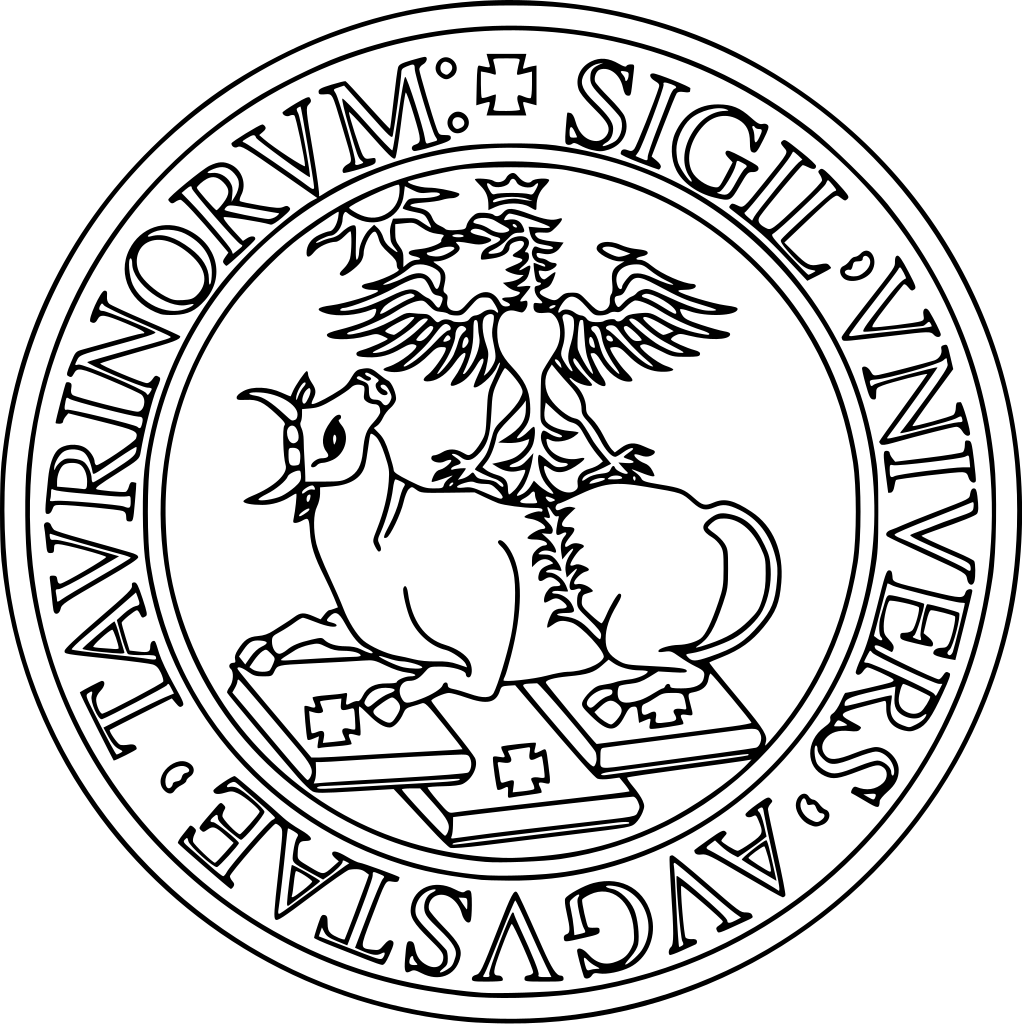
\includegraphics[width=5cm]{Immagini/logo.png}}


\vskip 1.2cm

\centerline {\normalsize {Tesi di Laurea Triennale}} 

\vskip 0.7cm

\centerline {\Large {\bf A FORMAL VERIFICATION}}

\vskip 0.3cm

\centerline {\Large {\bf OF REVERSIBLE PRIMITIVE PERMUTATIONS}}

\vskip 1.4cm

\noindent \textbf{Relatore:} Prof. Luca Roversi
\hfill  {\textbf{Candidato:} Giacomo Maletto }

\vskip 2.5cm

\centerline{2020/2021}

\section*{Abstract}

Proof assistants are computer programs designed to help with
the development of formal proofs.
In this thesis we explore this topic using the Lean theorem prover,
and by formalizing an article \cite{PAOLINI2020218} on reversible computing -
specifically, about a class of invertible computable functions called Reversible Primitive Permutations
which are expressive enough to encode the whole class of Primitive Recursive Functions.
In doing so, many aspects of the original paper are re-elaborated and simplified,
like the definition, the construction of the Cantor pairing and the proof of $\PRF$-completeness.

\tableofcontents

\mainmatter

\newpage

\chapter*{Introduction}
\markboth{Introduction}{INTRODUCTION}
\addcontentsline{toc}{chapter}{Introduction}


A peg puzzle can be an interesting toy for toddlers.
It usually consists of some wooden shapes which have to be
positioned in the appropriate hole - those shapes can look like animals, people or letters of the alphabet, for example.
If you have a dog block in your hand and you try to put it over the cat hole,
it's just not going to work. The pieces don't fit, it's \textit{physically impossible} to make it happen,
there's a mechanical barrier preventing it.

Mathematicians often like to pretend that they too are surrounded by mechanical barriers.
If a function is defined as $f : \NN \to \RR$ it's wrong to consider $f(-1)$,
by the inequalities $a < b$ and $a < c$ it doesn't follow in general that $b < c$,
if we write $2 + 2 = 5$ and consider this a correct equation over the natural numbers then we have made a mistake.
But it's not like the sheet of paper bursts into flames when such things are written on it -
so how do we know that there's something wrong?

By a complex process of recollection of past experiences, recognition of patterns,
discussion and exchange of ideas with others, and many other elements.
It's a very indirect process.

Not that there's anything necessarily wrong with this;
it can be argued that in mathematics, it's not the barriers that we put around us the important thing,
but rather what those barriers reveal and make us see more clearly.
Take group axioms (associativity, existence of the identity...): we don't really care about the axioms per se,
but rather what concepts they encapsulate and what emerges from those rules.
It's still possible to arrive at an important and insightful conclusion even if the path taken
is full of imprecisions, unjustified claims and even some mistakes:
who says that those mistakes might not turn into something new (for example, taking the square root of $-1$)?

Still, it's hard to deny that there's something inherently mechanical about mathematics.
Much of the development of math of the late 19th and 20th century is devoted to an effort to
cast everything in a solid ground. The current belief is that pretty much all mathematics can rest on Zermelo–Fraenkel set theory
with the axiom of choice, and that's a respectable intellectual position.
But the discipline keeps on being something nebulous, which exists in books and blackboards and the minds of people,
and sheets of paper still don't burn when we write down $2 + 2 = 5$; it's still something \textit{handcrafted}, a product of artisans.
\newpage
An alternative to this might be proof assistants.

A \textit{proof assistant} (or \textit{theorem prover}) is a computer software designed to help with
the development of formal proofs.
What this means, is that we can write down definitions, theorems and proofs about any sort of math on the computer,
and if there's something wrong it immediately lets us know.
The imaginary barriers that we previously constructed in our minds become
real, mechanical barriers - it becomes \textit{physically impossible} to put $-1$ as argument in $f : \NN \to \RR$,
or to provide an erroneous step inside a proof.

As a consequence, proof assistants give us (almost) absolute certainty about the things we write down on them,
which trace back directly to the "axioms" of the system in use.
Note that they do \textbf{not} automatically come up with proofs and concepts
(even if there's a lot of interest and work being put in this direction) but rather,
they offer us an environment in which our mathematical ideas can live in a very clear and precise form.

Systems like these run the risk of being far too pedantic and unwieldy to use,
but the recent development of large libraries of math in proof assistants such as Mizar, HOL, Coq and Lean
together with new landmark results (like the recent success of Peter Scholze's "liquid tensor experiment" \cite{quanta})
show us that they're getting better, and that it might be an interesting time to start using them.

\paragraph{}

In this thesis we wish to explore this new, fascinating field.
Our playground will be \textit{reversible computing} - specifically, a class of functions
called Reversible Primitive Permutations. We will present them alongside a promising, relatively new theorem prover
called Lean (together with its extensive and rapidly-growing community library, Mathlib),
in order to show the relationship between mathematical concepts and their computer formalization.


% a box full of variously shaped holes,
% together with some 
% 
% 
% A \textbf{proof assistant} or \textbf{theorem prover} 
% the development of formal proofs.
% These proofs can be about the correctness of algorithms and software,
% certifying that everything works correctly; or they can just be about pure math.

\chapter{The definition}

In this chapter we introduce mathematically the class of reversible primitive permutations
and then formalize its definition in Lean.

\section{Reversible computing}

Reversible computing is a model of computation in which every process can be run backwards \cite{Morita17}\cite{perumalla2013chc}.
Simply put, in a reversible setting any program takes inputs and gives outputs (like usual), but can also go the other way around:
provided the output it can reconstruct the input.
In a mathematical sense, every function is expected to be invertible.

Why do we care about such a thing?

Firstly, having a programming language in which every function (or even a subset of functions) is reversible could lead to interesting and practical applications.

But we can also imagine reversible computers, in which the underlying architecture is inherently reversible:
Toffoli gates provide a way to do so.
The opposite of reversibility is loss of information, which (for thermodynamic reasons) leads to loss of energy and heat dissipation.
This means that a non-reversible gate dissipates energy each time information is discarded, while in principle a reversible computer wouldn't.

Lastly, reversible computing is directly related to quantum computing, as each operation in a quantum computer must be reversible.


\section{Reversible Primitive Permutations}

In the article we decided to formalize \cite{PAOLINI2020218}, the authors focus on providing a functional model of reversible computation.
They develop an inductively defined set of functions, called \textbf{Reversible Primitive Permutations} or \textbf{RPP},
which are expressive enough to represent all Primitive Recursive Functions -
that is to say, $\RPP$ is $\PRF$-complete (we talk about what this means in section \ref{prfcompleteness}).
Here is the definition that we will use:

\newpage

\begin{definition}[Reversible Primitive Permutations]
\label{rppdef}
The class of \textbf{Reversible Primitive Permutations} or $\RPP$ is the smallest subset of functions $\ZZ^n \to \ZZ^n$ satisfying the following conditions:
\begin{itemize}

\item
The $n$-ary \textbf{identity} $\rppId_n (x_1, \dots, x_n) = (x_1, \dots, x_n)$ belongs to $\RPP$, for all $n \in \NN$.
\[\begin{NiceMatrix}[nullify-dots]
  x_1    & \bloch{3-1}{\rppId_n} & x_1    \\
  \Vdots &                       & \Vdots \\
  x_n    &                       & x_n    \\
\end{NiceMatrix}\]
The meaning of these diagrams should be fairly obvious:
if the values on the left of a function are provided as inputs to that function, we get the values on the right as outputs.
\item
The \textbf{sign-change} $\rppNe (x) = -x$ belongs to $\RPP$.
\[\begin{NiceMatrix}
  x & \bloch{1-1}{\rppNe} & -x \\
\end{NiceMatrix}\]

\item
The \textbf{successor function} $\rppSu (x) = x+1$ belongs to $\RPP$.
\[\begin{NiceMatrix}
  x & \bloch{1-1}{\rppSu} & x+1 \\
\end{NiceMatrix}\]

\item
The \textbf{predecessor function} $\rppPr (x) = x-1$ belongs to $\RPP$.
\[\begin{NiceMatrix}
  x & \bloch{1-1}{\rppPr} & x-1 \\
\end{NiceMatrix}\]

\item
The \textbf{swap} $\rppSw (x, y) = (y, x)$ belongs to $\RPP$.
\[\begin{NiceMatrix}
  x & \bloch{2-1}{\rppSw} & y \\
  y &                     & x \\
\end{NiceMatrix}\]

\item
If $f : \ZZ^n \to \ZZ^n$ and $g : \ZZ^n \to \ZZ^n$ belong to $\RPP$,
then the \textbf{series composition} $(f \rppCo g) : \ZZ^n \to \ZZ^n$ belongs to $\RPP$ and is such that:
\[(f \rppCo g) (x_1, \dots, x_n) = g (f (x_1, \dots, x_n)) = (g \circ f) (x_1, \dots, x_n).\]
We remark that $f \rppCo g$ means that $f$ is applied first, and then $g$, in opposition to the standard functional composition (denoted by $\circ$).
\[\begin{NiceMatrix}[nullify-dots]
  x_1    & \bloch{3-1}{f \rppCo g} & z_1    & \Block{3-1}{=} & x_1    & \bloch{3-1}{f} & y_1    & \bloch{3-1}{g} & z_1    \\
  \Vdots &                         & \Vdots &                & \Vdots &                & \Vdots &                & \Vdots \\
  x_n    &                         & z_n    &                & x_n    &                & y_n    &                & z_n    \\
\end{NiceMatrix}\]

\item

If $f : \ZZ^n \to \ZZ^n$ and $g : \ZZ^m \to \ZZ^m$ belong to $\RPP$,
then the \textbf{parallel composition} $(f \rppPa g) : \ZZ^{n + m} \to \ZZ^{n + m} $ belongs to $\RPP$ and is such that:
\[(f \rppPa g) (x_1, \dots, x_n, y_1, \dots, y_m) = (f (x_1, \dots, x_n), g (y_1, \dots, y_m)).\]
\[\begin{NiceMatrix}[nullify-dots]
  x_1    & \bloch{6-1}{f \rppPa g} & z_1    & \Block{6-1}{=} & x_1    & \bloch{3-1}{f} & z_1    \\
  \Vdots &                         & \Vdots &                & \Vdots &                & \Vdots \\
  x_n    &                         & z_n    &                & x_n    &                & z_n    \\
  y_1    &                         & w_1    &                & y_1    & \bloch{3-1}{g} & w_1    \\
  \Vdots &                         & \Vdots &                & \Vdots &                & \Vdots \\
  y_m    &                         & w_m    &                & y_m    &                & w_m    \\
\end{NiceMatrix}\]

\item
If $f : \ZZ^n \to \ZZ^n$ belongs to $\RPP$,
then then \textbf{finite iteration} $\rppIt[f] : \ZZ^{n + 1} \to \ZZ^{n + 1}$ belongs to $\RPP$ and is such that:
\[ \rppIt[f] (x, x_1, \dots, x_n) = (x, (\overbrace{f \circ \dots \circ f}^{\downarrow x \text{ times}}) (x_1, \dots, x_n)) \]
where $\downarrow (\cdot) : \ZZ \to \NN$ is defined as
\[\downarrow x = \begin{cases} x, & \text{if $x \ge 0$} \\
                               0, & \text{if $x < 0$} \end{cases}.\]
This means that the function $f$ is applied $\downarrow x$ times to $(x_1, \dots, x_n)$.
\[\begin{NiceMatrix}[nullify-dots]
  x      & \bloch{4-1}{\rppIt[f]} & x      & \Block{4-1}{=} & x      &                                                                       &                    &                & x      \\  
  x_1    &                        & y_1    &                & x_1    & \bloch{3-1}{f}                                                        & \Block{3-1}{\dots} & \bloch{3-1}{f} & y_1    \\
  \Vdots &                        & \Vdots &                & \Vdots &                                                                       &                    &                & \Vdots \\
  x_n    &                        & y_n    &                & x_n    &                                                                       &                    &                & y_n    \\
         &                        &        &                &        & \Block{1-3}{\underbrace{\hspace{5.5em}}_{\downarrow x \text{ times}}} &                    &                &        \\
\end{NiceMatrix}\]

\item
If $f, g, h : \ZZ^n \to \ZZ^n$ belong to $\RPP$,
then the \textbf{selection} $\rppIf[f, g, h] : \ZZ^{n + 1} \to \ZZ^{n + 1}$ belongs to $\RPP$ and is such that:
\[\rppIf[f, g, h] (x, x_1, \dots, x_n) = \begin{cases} (x, f (x_1, \dots, x_n)), & \text{if $x > 0$} \\
                                                    (x, g (x_1, \dots, x_n)), & \text{if $x = 0$} \\
                                                    (x, h (x_1, \dots, x_n)), & \text{if $x < 0$} \end{cases}.\]
We remark that the argument $x$ which determines which among $f$, $g$ and $h$ must be used cannot be among the arguments of $f$, $g$ and $h$,
as that would break reversibility.
\[\begin{NiceMatrix}[nullify-dots]
  x      & \bloch{4-1}{\rppIf[f, g, h]} & x      \\
  x_1    &                              & y_1    \\
  \Vdots &                              & \Vdots \\
  x_n    &                              & y_n    \\
\end{NiceMatrix} \quad
\begin{NiceMatrix}[nullify-dots]
                 &                     &                  \\
  \Block{3-1}{=} & f (x_1, \dots, x_n) & \text{if } x > 0 \\
                 & g (x_1, \dots, x_n) & \text{if } x = 0 \\
                 & h (x_1, \dots, x_n) & \text{if } x < 0 \\
\CodeAfter
\SubMatrix\}{2-1}{4-1}\{  
\end{NiceMatrix}\]

\end{itemize}
\end{definition}

\begin{remark}
\label{different_arity}
If we have two functions of different arity, for example $f : \ZZ^3 \to \ZZ^3$ and $g : \ZZ^5 \to \ZZ^5$,
then we will still write $f \rppCo g$ to mean the function with arity $\max(3, 5)=5$ given by $(f \rppPa \rppId_2) \rppCo g$.
In general, the arity of the "smaller" function can be enlarged by a suitable parallel composition with the identity.
The same goes for the arguments of the selection $\rppIf[f, g, h]$.
\[\begin{NiceMatrix}[nullify-dots]
  x_1 & \bloch{5-1}{f \rppCo g} & z_1 & \Block{5-1}{=} & x_1 & \bloch{3-1}{f} & y_1 & \bloch{5-1}{g} & z_1 & \Block{5-1}{=} & x_1 & \bloch{3-1}{f}        & y_1 & \bloch{5-1}{g} & z_1 \\
  x_2 &                         & z_2 &                & x_2 &                & y_2 &                & z_2 &                & x_2 &                       & y_2 &                & z_2 \\
  x_3 &                         & z_3 &                & x_3 &                & y_3 &                & z_3 &                & x_3 &                       & y_3 &                & z_3 \\
  x_4 &                         & z_4 &                & x_4 &                & x_4 &                & z_4 &                & x_4 & \bloch{2-1}{\rppId_2} & x_4 &                & z_4 \\
  x_5 &                         & z_5 &                & x_5 &                & x_5 &                & z_5 &                & x_5 &                       & x_5 &                & z_5 \\
\end{NiceMatrix}\]
\end{remark}


\section{Some examples}

In order to get accustomed to this definition, let's see some examples.

\paragraph{Increment and decrement}
Let's try to imagine what addition should look like in $\RPP$.
Of course, addition is usually thought of as a function which takes two inputs and yields their sum:
something like $\texttt{add}(x,y) = x+y$.
But notice that this operation is not reversible:
given only the output (the value $x+y$) it is impossible to obtain the original values ($x, y$).
As we will see, every function in $\RPP$ is reversible, so we will not be able to define addition in this way.

Instead, we can define a function $\rppinc$ in $\RPP$ which, given $n \in \NN$ and $x \in \ZZ$, yields
\[\begin{NiceMatrix}
  n & \bloch{2-1}{\rppinc} & n     \\
  x &                      & x + n \\
\end{NiceMatrix}\]
If $n$ is negative the output is just $(n, x)$.
The fact that the above diagram is only valid for $n \in \NN$ might bother some readers;
we'll explain later why it is so, and how we can also make it work for $n \in \ZZ$.

For now let's focus on the output: we don't just have $x + n$ but also $n$, and indeed,
given both $n$ and $x+n$ we can reconstruct $n$ (obviously) and $x$ (by $(x+n)-n$).
As a matter of fact, the following function $\rppdec$ also belongs to $\RPP$:
\[\begin{NiceMatrix}
  n & \bloch{2-1}{\rppdec} & n     \\
  x &                      & x - n \\
\end{NiceMatrix}\]
and if we try to compose $\rppinc$ and $\rppdec$ we get this remarkable result:
\[\begin{NiceMatrix}
  n & \bloch{2-1}{\rppinc} & n     & \bloch{2-1}{\rppdec} & n \\
  x &                      & x + n &                      & x \\
\end{NiceMatrix}\]
and similarly for $\rppdec \rppCo \rppinc$.
So indeed $\rppdec$ is the inverse of $\rppinc$, and we can write $\rppdec = \rppinc^{-1}$.

But we haven't said how to actually define $\rppinc$.
Well, just like this:
\[\rppinc = \rppIt[\rppSu]\]
This means that we apply the successor function $\rppSu$ to the value $x$, for $\downarrow n$ times.
If $n \in \NN$ then $\downarrow n = n$, so we effectively add $n$ to the value $x$.
If instead $n$ is negative then $\downarrow n = 0$ and nothing changes.

Can the reader guess how $\rppdec$ is defined?
\newpage
In a very similar manner, using the predecessor function:
\[\rppdec = \rppIt[\rppPr]\]
and as we will shortly see, finding the inverse is not something that we have to do by hand.

\paragraph{Multiplication and square}
We now turn our attention to multiplication.
The elementary-school way to define multiplication is by repeated addition, and we can define $\rppmul$ exactly like that:
\[\rppmul = \rppIt[\rppinc].\]
As $\rppinc$ had arity $2$, $\rppmul$ has arity $2+1=3$.
If $n, m \in \NN$ and $x \in \ZZ$ then we have
\[\begin{NiceMatrix}
  n & \bloch{3-1}{\rppmul} & n             \\
  m &                      & m             \\
  x &                      & x + n \cdot m \\
\end{NiceMatrix}\]
because we're essentially "incrementing by $m$" $n$ times;
so in this case we preserve both inputs and increase a certain variable $x$.

What is the inverse $\rppmul^{-1}$? Does it perform division?
Well, the truth is rather disappointing:
\[\begin{NiceMatrix}
  n & \bloch{3-1}{\rppmul^{-1}} & n             \\
  m &                           & m             \\
  x &                           & x - n \cdot m \\
\end{NiceMatrix}\]
We will see a way to calculate division in $\RPP$, but this is not it.

We're now ready to define the function $\rppsquare$ which is used to calculate the square of a number:
\[\rppsquare = (\rppId_1 \rppPa \rppSw) \rppCo \rppinc \rppCo \rppmul \rppCo \rppdec \rppCo (\rppId_1 \rppPa \rppSw).\]
That might look like a very complicated expression;
thankfully we can make use of diagrams to show what each step does.
Given $n \in \NN$ and $x \in \ZZ$ we have
\[\begin{NiceMatrix}
  n &                     & n & \bloch{2-1}{\rppinc} & n & \bloch{3-1}{\rppmul} & n             & \bloch{2-1}{\rppdec} & n             &                     & n             \\
  x & \bloch{2-1}{\rppSw} & 0 &                      & n &                      & n             &                      & 0             & \bloch{2-1}{\rppSw} & x + n \cdot n \\
  0 &                     & x &                      & x &                      & x + n \cdot n &                      & x + n \cdot n &                     & 0             \\
\end{NiceMatrix}\]
so we add the result $n \cdot n$ to a variable $x$;
we also require an additional value initialized to 0.
We will make frequent use of variables initially set to 0 and which come back to 0 after the calculation;
these are traditionally called \textbf{ancillary arguments} or \textbf{ancillaes}, from the latin term used to describe female house slaves in ancient Rome.

The reader might be wondering what would happen if $n < 0$ or the ancilla was different from $0$.
The truth is, we don't really care.
We will often specify the behaviour of these functions given some initial values,
and we won't need to know what happens for different initial values because we'll never use those functions in other ways.

\section{Calculating the inverse}

Earlier we hinted at the fact that every function in $\RPP$ is invertible and the inverse belongs to $\RPP$;
furthermore, we don't need to perform the calculation manually, case by case.
In other words, there is an \textit{effective procedure} which produces the inverse $f^{-1} \in \RPP$ given any $f \in \RPP$.

\begin{proposition}[The inverse $f^{-1}$ of any $f$]
\label{rppinv}
Let $f : \ZZ^n \to \ZZ^n$ belong to $\RPP$.
Then the inverse $f^{-1} : \ZZ^n \to \ZZ^n$ exists, belongs to $\RPP$ and, by definition, is
\begin{itemize}
\item $\rppId_n^{-1} = \rppId_n$
\item $\rppNe^{-1} = \rppNe$
\item $\rppSu^{-1} = \rppPr$
\item $\rppPr^{-1} = \rppSu$
\item $\rppSw^{-1} = \rppSw$
\item $(f \rppCo g)^{-1} = g^{-1} \rppCo f^{-1}$
\item $(f \rppPa g)^{-1} = f^{-1} \rppPa g^{-1}$
\item ${\rppIt[f]}^{-1} = \rppIt[f^{-1}]$
\item ${\rppIf[f, g, h]}^{-1} = \rppIf [f^{-1}, g^{-1}, h^{-1}]$
\end{itemize}
Then $f \rppCo f^{-1} = \rppId_n$ and $f^{-1} \rppCo f = \rppId_n$.
\end{proposition}
\begin{proof}
By induction on the definition of $f$.
\end{proof}

Well, that was rather succinct.

We invite the reader to check that every listed inverse does indeed make sense;
for example, the function $\rppIt[f] (x, y_1, \dots, y_n)$ applies $\downarrow x$ times the function $f$ to the argument $(y_1, \dots, y_n)$.
If we want to "undo" this effect we just need to apply $\downarrow x$ times $f^{-1}$ to the same argument, so
${\rppIt[f]}^{-1} = \rppIt[f^{-1}]$.

Of course, that reasoning only works if in turn $f$ is also invertible and $f^{-1} \in \RPP$.
This is the reason that the proof is by induction:
given an arbitrary $\RPP$, if we unfold one step of the definition we get one of the cases listed.
We apply the appropriate step and then by inductive hypothesis we can assume that in turn its sub-terms are invertible.

Notice that in this way, if we try to calculate $\rppinc^{-1}$ we really do get $\rppdec$, as we had hoped for.

Since $\RPP$ is inductively defined, any proposition involving $\RPP$ functions can be proven using induction.
Not only that, but any function which has for an argument a generic $\RPP$ can be defined recursively,
and indeed we can also see $(\cdot)^{-1}:\RPP \to \RPP$ as a recursive function.
In section \ref{curry} we will see that induction and recursion can be seen as really the same thing,
and that's just one of many similarities between functions and proofs.

\section{First steps with Lean}

In this section we take a look at some of Lean's basic features.

In Lean we primarily do three things:
\begin{enumerate}
\item define data structures
\item define functions
\item prove theorems about data structures and functions
\end{enumerate}
What sets Lean apart from your average functional programming language (like Haskell) is the third item on the list.
Now we will instead focus on the first and second points.

The reader isn't expected to understand every detail of what will follow -
a vague understanding of what's going on would be sufficient.
Most of the following snippets of code can be run and played with
in the online editor\footnote{\url{https://leanprover-community.github.io/lean-web-editor/}.},
while those pertaining $\RPP$ require more set-up\footnote{The code can be found at \url{https://github.com/GiacomoMaletto/RPP/tree/main/Lean},
and uses Mathlib \cite{mathlib}.}.

\paragraph{A simple example of type}
Data is defined using the \lstinline{inductive} keyword.
Here is the typical example of data structure \cite{theoremprovinglean}:
\begin{lstlisting}
inductive weekday : Type
| monday : weekday
| tuesday : weekday
| wednesday : weekday
| thursday : weekday
| friday : weekday
| saturday : weekday
| sunday : weekday
\end{lstlisting}
This defines a \textit{type} called \lstinline{weekday}.
Days of the week like \lstinline{monday}, \lstinline{tuesday}, etc. are elements of the type \lstinline{weekday}.
We can see the type of an element by using the \lstinline{#check} command:
\begin{lstlisting}
-- opening the scope weekday (otherwise to refer
-- to an element - for example tuesday - of weekday
-- we have to write weekday.tuesday)
open weekday

#check tuesday -- this outputs "weekday"
\end{lstlisting}
and we write this as
\begin{lstlisting}
tuesday : weekday
\end{lstlisting}
Everything in Lean has a type (and only one). For example, natural numbers have type \lstinline{ℕ}:
\begin{lstlisting}
#check 3 -- ℕ
\end{lstlisting}
Even type themselves have a type\footnote{Types in Lean have a role similar to sets in math.
Standard math axioms (like ZFC) dictates that everything is a set, including sets themselves.
This basic notion can lead to some contradictory statements, like the famous Russell's paradox
(let's consider the set of all sets that do not contain themselves; does this set contain itself?)
and if one is not careful in defining types of types, the same thing could happen with type theory.
But in fact, type theory was invented in the beginning of the 20th century by Bertrand Russell precisely to avoid Russell's paradox.
The approach used in Lean is to define a cumulative hierarchy of universes \lstinline{Type : Type 1 : Type 2 ...},
so that it's impossible to invoke objects like "the type of all types" or a type having itself as an element. \cite{CarneiroMaster}}.
Lean's type system is very expressive, and makes it possible to work with complex math in Lean.

We can define functions over the type \lstinline{weekday} -
for example, the function \lstinline{next}:

\begin{lstlisting}
-- Special characters like → will abound.
-- In VS Code and the Lean Web Editor,
-- arrows can be inserted by typing \to and hitting
-- the space bar. 
def next : weekday → weekday
| monday    := tuesday
| tuesday   := wednesday
| wednesday := thursday
| thursday  := friday
| friday    := saturday
| saturday  := sunday
| sunday    := monday

#reduce next wednesday -- this outputs "thursday"
#check next -- next has type "weekday → weekday"
\end{lstlisting}
This function is defined by cases:
if we have \lstinline{monday}, output \lstinline{tuesday},
if we have \lstinline{tuesday}, output \lstinline{wednesday}, and so on.

(Almost \cite{CarneiroMaster}) every expression - like \lstinline{next (next thursday)} or \lstinline{3 * 5 + 2} -
have a corresponding \textit{reduced form} (respectively \lstinline{saturday} and \lstinline{17})
which can be displayed using the \lstinline{#reduce} command,
and is obtained by repeatedly applying functions to their arguments, until the full computation is carried out.
In this sense, things like \lstinline{next wednesday} and \lstinline{next (next tuesday)}
(or \lstinline{2 + 2} and \lstinline{1 + 3}) are \textit{definitionally equivalent}, because they're reduced to the same expression.

An important remark on notation:
in math it is customary to call functions by enclosing arguments in parenthesis and separating them with commas, i.e. $f(x,y,z)$.
Languages like Lean follow a different convention: the arguments are simply written after the function name, like \lstinline{f x y z}.
So in our case, what we would write as $\mathsf{next(next(thursday))}$ is instead written \lstinline{next (next thursday)}
(writing \lstinline{next next thursday} would be wrong
because it would mean that the first argument to \lstinline{next} is the function \lstinline{next} itself, not \lstinline{next thursday}).
This doesn't lead to ambiguity and often helps reducing clutter.

\paragraph{An example of inductive type}
Right now the reader could be wondering why we used the keyword \lstinline{inductive} to define \lstinline{weekday},
when there's \textit{clearly} no induction going on at all in its construction.
First of all, it depends on what is meant by induction; but it is true that that was a particularly simple case.
As an example of a more overtly inductive object, we can define the natural numbers like this:
\begin{lstlisting}
inductive Nat : Type
| Zero : Nat
| Succ (n : Nat) : Nat
\end{lstlisting}
The name \lstinline{Nat} and subsequent objects are capitalized in order to avoid conflict with the definition of \lstinline{nat} already present in Lean.
We can read this definition as "every element of the type \lstinline{Nat} is either \lstinline{Zero}
or \lstinline{Succ n} where \lstinline{n : Nat}",
which is basically the Peano definition of natural numbers.
Some examples of elements of this type:
\begin{lstlisting}
open Nat

-- all these outputs "Nat"
#check Zero -- represents 0
#check Succ Zero -- represents 1
#check Succ (Succ Zero) -- represents 2
#check Succ (Succ (Succ Zero)) -- represent 3
#check Zero.Succ.Succ.Succ -- also represents 3
                           -- alternative notation
\end{lstlisting}
Functions over \lstinline{Nat} have the possibility of being truly recursive:
for example, we can recursively define addition \lstinline{Add m n} by induction over \lstinline{n}.
\begin{itemize}
\item if \lstinline{n = Zero} then \lstinline{Add m Zero = m}
\item if \lstinline{n = Succ n'} for some \lstinline{n' : Nat}, \\
      then \lstinline{Add m (Succ n') = Succ (Add m n')}.
\end{itemize}
Note that by definition each element of \lstinline{Nat} can be either \lstinline{Zero} or \lstinline{Succ n'} for some \lstinline{n' : Nat},
so the two cases considered cover all possibilities.
Written in Lean,
\begin{lstlisting}
def Add : Nat → Nat → Nat
| m Zero      := m
| m (Succ n') := Succ (Add m n')
\end{lstlisting}
It may have struck you that the type of \lstinline{Add} is not \lstinline{Nat × Nat → Nat}
but instead \lstinline{Nat → Nat → Nat}.
This is known as \textit{currying}, and it's not as strange as it might look like at first.
Consider this: we can think of \lstinline{Add} as a function which takes a pair \lstinline{(m,n) : Nat × Nat} and outputs \lstinline{Add m n : Nat},
as is standard in mathematics.
But we can also think of it as a function which takes just \lstinline{m : Nat} and outputs the function \lstinline{Add m : Nat → Nat},
which in turn given \lstinline{n : Nat} outputs \lstinline{Add m n : Nat}.
We can think of \lstinline{Add m} as a partially applied function, which becomes fully applied when it is given another argument \lstinline{n}.
From this point of view, \lstinline{Add} is a function of type \lstinline{Nat → (Nat → Nat)} which is the same as
\lstinline{Nat → Nat → Nat} because in Lean the arrow \lstinline{→} is right associative.

In a certain sense, currying makes functions conceptually simpler;
all functions are single variable, it's just that some return other functions.

\paragraph{Integers and lists}
Functions belonging to $\RPP$ have $\ZZ^n$ as their domain and codomain,
so we need a way to represent and work with integer tuples.

The good news is that integers are already defined in Lean\footnote{Deciding how to define something like the integers in
a proof assistant is not so obvious - there are many equivalent ways,
but some are more convenient than others. For a comparison see \cite{ints}}.
Here is their definition:
\begin{lstlisting}
inductive int : Type
| of_nat (n : ℕ) : int
| neg_succ_of_nat (n : ℕ) : int  
\end{lstlisting}
The value \lstinline{of_nat n} represents the natural number \lstinline{n : ℕ} as an integer,
while \lstinline{neg_succ_of_nat n} represents the negative number \lstinline{-(n+1)}.
Of course it's not the definition we've just seen that gives this meaning to the \lstinline{int}s;
rather, it's the functions defined on them (like addition, subtraction etc.).

Immediately after the definition, some notation is introduced:
\begin{itemize}
\item \lstinline{ℤ} stands for \lstinline{int}
\item in a context in which an integer is expected, if instead a natural number is supplied,
the function \lstinline{of_nat} will be automatically applied on the natural number.
This convenient feature is called coercion.
\item for every \lstinline{n : ℕ}, \lstinline{-[1+ n]} stands for \lstinline{neg_succ_of_nat n}.
This notation is almost never used.
\end{itemize}
\begin{lstlisting}
notation `ℤ` := int

instance : has_coe nat int := ⟨int.of_nat⟩

notation `-[1+ ` n `]` := int.neg_succ_of_nat n
\end{lstlisting}
As an example of a function from \lstinline{ℤ} to \lstinline{ℤ}, this is negation:
\begin{lstlisting}
def neg : ℤ → ℤ
| (of_nat n) := neg_of_nat n
| -[1+ n]    := succ n
\end{lstlisting}

We're interested not just in integers, but in tuples of integers.
We can implement the concept of a tuple in many ways,
but a particularly simple one is through the use of lists,
a very common data structure in computer science.

Let's consider lists of natural numbers, i.e. the type \lstinline{list ℕ}.
This is a list of 5 elements:
\begin{lstlisting}
open list
#reduce [4, 5, 7, 2, 5] -- [4, 5, 7, 2, 5]
\end{lstlisting}
The first element of a list is the \textit{head}
\begin{lstlisting}
#reduce head [4, 5, 7, 2, 5] -- 4
\end{lstlisting}
while the other elements are the \textit{tail}.
\begin{lstlisting}
#reduce tail [4, 5, 7, 2, 5] -- [5, 7, 2, 5]
\end{lstlisting}
Given \lstinline{n : ℕ} and \lstinline{X : list ℕ} we can obtain a new list
\lstinline{cons n X} (also written as \lstinline{n :: X}) such that
\lstinline{head (n :: X) = n} and \lstinline{head (n :: X) = X}
\begin{lstlisting}
#reduce cons 2 [4, 5, 7, 2, 5] -- [2, 4, 5, 7, 2, 5]
#reduce 2 :: [4, 5, 7, 2, 5]   -- alternative notation  
\end{lstlisting}
and ultimately, every list can be obtained by starting with \lstinline{nil},
the empty list, and repeatedly using \lstinline{cons}.
\begin{lstlisting}
#reduce nil -- the empty list
#reduce []  -- alternative notation 
#reduce cons 4 (cons 5 (cons 7 (cons 2 (cons 5 nil))))
            -- [4, 5, 7, 2, 5]
#reduce 4 :: 5 :: 7 :: 2 :: 5 :: []
            -- alternative notation
\end{lstlisting}
This might suggest a definition of lists of naturals:
a \lstinline{list_nat} is either the empty list \lstinline{nil_nat},
or \lstinline{cons_nat hd tl} where \lstinline{hd : ℕ} and \lstinline{tl : list_nat}
are respectively the head and tail of the list:
\begin{lstlisting}
inductive list_nat : Type
| nil_nat : list_nat
| cons_nat (hd : ℕ) (tl : list_nat) : list_nat
\end{lstlisting}
There's nothing special about using natural numbers.
We can use the same procedure to define lists of integers:
\begin{lstlisting}
inductive list_int : Type
| nil_int : list_int
| cons_int (hd : ℤ) (tl : list_int) : list_int
\end{lstlisting}
but having to define different types of lists for each type of element is pretty cumbersome.
Instead, we can define lists for a generic type \lstinline{T} using \textit{dependent types}:\footnote{a Lean user would probably frown at this,
because it would be best to choose an explicit universe \lstinline{u} and work with \lstinline{Type u}.}
\begin{lstlisting}
inductive list (T : Type) : Type
| nil : list
| cons (hd : T) (tl : list) : list
\end{lstlisting}
Rather than having \lstinline{list_nat}, \lstinline{list_int}...
we use \lstinline{list ℕ}, \lstinline{list ℤ}...
\lstinline{list α} where \lstinline{α} is any type.

We can see how useful dependent types are by defining the function \lstinline{length}
which returns the number of elements of a list:
\begin{lstlisting}
def length {α : Type*} : list α → ℕ
| []       := 0
| (a :: X) := length X + 1
\end{lstlisting}
Note that we can use \lstinline|{α : Type*}| to refer to a generic type \lstinline{α}.
If instead we had stuck to \lstinline{list_nat}, \lstinline{list_int}...
now we would have to define \lstinline{length_nat}, \lstinline{length_int}... separately for each type.

We will identity tuples of $n$ elements $\ZZ^n$ with lists in \lstinline{list ℤ} of length \lstinline{n}.

\section{The definition in Lean}

\paragraph{Syntax and semantics}
Let's now ask ourselves: how can we define in a satisfactory way the class of functions $\RPP$ in Lean,
using just types and functions?
We'd like to be able to do proofs by induction over $\RPP$, like in proposition \ref{rppinv}, so we'll need to define an inductive type.

The key is thinking about $\RPP$ not as a class of functions, but as a small programming language.
In this sense, we can write down "programs" like our square function
\[(\rppId_1 \rppPa \rppSw) \rppCo \rppinc \rppCo \rppmul \rppCo \rppdec \rppCo (\rppId_1 \rppPa \rppSw)\]
but we should not view it only as a function belonging to $\ZZ^3 \to \ZZ^3$,
but also as the sentence
"$(\rppId_1 \rppPa \rppSw) \rppCo \rppinc \rppCo \rppmul \rppCo \rppdec \rppCo (\rppId_1 \rppPa \rppSw)$"
which can then be interpreted as the mathematical function belonging to $\ZZ^3 \to \ZZ^3$.

We thus separate between the \textit{syntax} and the \textit{semantics} of our language.
\begin{itemize}
\item The syntax are the rules which governs how to assemble well-structured sentences.
For example, the selection symbol $\rppIf$ should be followed by three other $\RPP$ functions;
if we write $\rppIf[\rppSu, \rppPr] \rppCo \rppNe$ we get a non-valid sentence.
\item The semantics is the meaning we give to (well-structured) sentences -
in our case, they are intepreted as functions $\ZZ^n \to \ZZ^n$.
\end{itemize}

A possible way to define $\RPP$ functions in Lean is
\begin{itemize}
\item define the type $\RPP$ which has for elements syntactically-correct sentences of $\RPP$
\item define a function $\mathsf{evaluate} : \RPP \to (\ZZ^n \to \ZZ^n)$ which assigns to each $\RPP$-sentence its intended meaning,
namely a function $\ZZ^n \to \ZZ^n$.
\end{itemize}
Note that this is not the only way in which this task can be accomplished;
we will discuss other methods in section \ref{alternatives}.

We thus define the type $\RPP$ as follows:
\begin{lstlisting}
inductive RPP : Type
| Id (n : ℕ) : RPP
| Ne : RPP
| Su : RPP
| Pr : RPP
| Sw : RPP
| Co (f g : RPP) : RPP
| Pa (f g : RPP) : RPP
| It (f : RPP) : RPP
| If (f g h : RPP) : RPP
\end{lstlisting}
and also introduce custom notation:
\begin{lstlisting}
-- the numbers 50 and 55 denote the precedence -
-- simply put, Ne ;; Su ‖ Pr is intepreted as
-- Ne ;; (Su ‖ Pr), not (Ne ;; Su) ‖ Pr
infix `;;` : 50 := Co
infix `‖` : 55 := Pa -- \Vert ‖
\end{lstlisting}
so it's now possible to write expressions like
\begin{lstlisting}
#check It Su ;; (Id 2 ‖ If Sw Pr Su) -- RPP
\end{lstlisting}
Remember that by remark \ref{different_arity}, it makes sense to consider the series composition of functions of different arity,
as long as we give them the meaning specified in the remark.

Talking about arity, how do we deal with it?
In order to define $\mathsf{evaluate}$ and give meaning to $\RPP$,
we must be able to define a concept of arity,
otherwise we'll have trouble with parallel composition of two functions \lstinline{f ‖ g} -
the arity of \lstinline{f} must be known,
otherwise it's impossible to tell what to apply \lstinline{g} to.

Luckily, we can reconstruct the arity of an \lstinline{RPP} just by looking at its symbolic representation:
\begin{lstlisting}
def arity : RPP → ℕ
| (Id n)     := n
| Ne         := 1
| Su         := 1
| Pr         := 1
| Sw         := 2
| (f ;; g)   := max f.arity g.arity
| (f ‖ g)    := f.arity + g.arity
| (It f)     := f.arity + 1
| (If f g h) := max (max f.arity g.arity) h.arity + 1
\end{lstlisting}
Note that \lstinline{f.arity} is the same as \lstinline{(arity f)}.
This is a recursive function:
there are 5 base cases and in the other 4 the value of \lstinline{arity} is reconstructed from smaller sub-terms.

It's now possible to define some \lstinline{RPP}-sentences in Lean
\begin{lstlisting}
def Id₁ := Id 1 -- ₁ \1
def inc := It Su
def dec := It Pr
def mul := It inc
def square := Id₁ ‖ Sw ;; inc ;; mul ;; dec ;; Id₁ ‖ Sw
\end{lstlisting}
and it's even possible to calculate their arity
\begin{lstlisting}
#reduce square.arity -- outputs "3"
\end{lstlisting}
but we haven't yet given their meaning as functions.

\paragraph{The \lstinline{ev} function}
We are now ready to define \lstinline{evaluate} (\lstinline{ev} for short).
The function $\mathsf{ev}$ should take $\RPP$-sentences and return functions $\ZZ^n \to \ZZ^n$,
so in Lean we will define it as a function of type
\begin{lstlisting}
RPP → (list ℤ → list ℤ)
\end{lstlisting}
which in Lean is the same as
\begin{lstlisting}
RPP → list ℤ → list ℤ.
\end{lstlisting}
Here's how we do it:
\begin{lstlisting}
def ev : RPP → list ℤ → list ℤ
| (Id n)     X                    := X
| Ne         (x :: X)             := -x :: X
| Su         (x :: X)             := (x + 1) :: X
| Pr         (x :: X)             := (x - 1) :: X
| Sw         (x :: y :: X)        := y :: x :: X
| (f ;; g)   X                    := ev g (ev f X)
| (f ‖ g)    X                    := ev f (take f.arity X) ++
                                     ev g (drop f.arity X)
| (It f)     (x :: X)             := x :: ((ev f)^[↓x] X)
| (If f g h) (0 :: X)             := 0 :: ev g X
| (If f g h) (((n : ℕ) + 1) :: X) := (n + 1) :: ev f X
| (If f g h) (-[1+ n] :: X)       := -[1+ n] :: ev h X
| _          X                    := X

notation `‹` f `›` := ev f -- ‹ \f › \fr
\end{lstlisting}
We will write \lstinline{‹f›} to mean the function of type \lstinline{list ℤ → list ℤ} given by \lstinline{ev f}.

Here's a case-by-case analysis:
\begin{itemize}
\item \lstinline{‹Id n› X} is the original list \lstinline{X}, unchanged.
\item \lstinline{‹Ne› (x :: X)} reduces to \lstinline{-x :: X}, which is same list but with the head of opposite sign.
\item \lstinline{‹Su› (x :: X)} reduces to the same list but with the head incremented by one.
\item \lstinline{‹Pr› (x :: X)} reduces to the same list but with the head decremented by one.
\item \lstinline{‹Sw› (x :: y :: X)} reduces to the same list but with the first two elements swapped.
\item \lstinline{‹f ;; g› X} successively applies \lstinline{‹f›} and \lstinline{‹g›} to the list.
\item \lstinline{‹f ‖ g› X} applies \lstinline{‹f›} to the first \lstinline{f.arity} elements of the list,
applies \lstinline{‹g›} to the remaining elements of the list,
and then joins the two parts through \lstinline{append} (which is the \lstinline{(++)} operator).
\item \lstinline{‹It f› (x :: X)} leaves the head unchanged and applies \lstinline{‹f›} to the tail \lstinline{↓x} times,
where \lstinline{↓x} is defined as in definition \ref{rppdef}.
\item \lstinline{‹If f g h› (0 :: X)} leaves the head unchanged and applies \lstinline{‹g›} to the tail.
\item \lstinline{‹If f g h› (((n : ℕ) + 1) :: X)} is the case where the head is a positive number
(a natural number plus \lstinline{1}),
and as such leaves the head unchanged and applies \lstinline{‹f›} to the tail.
\item \lstinline{‹If f g h› (-[1+ n] :: X)} is the case where the head is a negative number,
and as such leaves the head unchanged and applies \lstinline{‹h›} to the tail.
\item In all cases not considered (for example, applying \lstinline{‹Ne›} to an empty list) the whole list remains unchanged. 
\end{itemize}

The reader is invited to compare this definition with the one given in definition \ref{rppdef}.

Let's see some examples:
\begin{lstlisting}
#check ‹It Su ;; (Id₁ ‖ If Sw Pr Su)› -- list ℤ → list ℤ
-- #eval is similar to #reduce
-- but in this case gives more readable output
#eval ‹inc› [3, 4] -- [3, 7]
#eval ‹square› [19, 0, 0] -- [19, 361, 0]
\end{lstlisting}
It magically works. We finally have our definition formalized in Lean.

It is worth noting that even though lists supplied to \lstinline{‹f›} are supposed to have length equal to \lstinline{f.arity},
this is never enforced.
So we are free to apply \lstinline{‹f›} to a list which is too short or too long.
If it's too short, unspecified things will happen, we don't care.
If it's too long, only the first \lstinline{f.arity} items are utilized and affected,
and this is guaranteed by theorem \lstinline{ev_split} which we will prove in Lean.
So, when we apply \lstinline{RPP} functions to a list, we'll have to make sure that
\lstinline{f.arity ≤ X.length}.

\paragraph{The \lstinline{inverse} function}
It's not hard to convert our proposition \ref{rppinv} into a function definition:
\lstinline{inv : RPP → RPP} which given \lstinline{f : RPP} returns its inverse.
\begin{lstlisting}
def inv : RPP → RPP
| (Id n)     := Id n
| Ne         := Ne
| Su         := Pr
| Pr         := Su
| Sw         := Sw
| (f ;; g)   := inv g ;; inv f
| (f ‖ g)    := inv f ‖ inv g
| (It f)     := It (inv f)
| (If f g h) := If (inv f) (inv g) (inv h)

notation f `⁻¹` := inv f -- ⁻¹ \-1
\end{lstlisting}
Now it's possible to define \lstinline{dec} simply as \lstinline{inc⁻¹}.

We will also prove in Lean that \lstinline{f⁻¹} really is the inverse (in the functional sense) of \lstinline{f},
but it will require some work.
\section{Differences with the original definition}
The definition of \lstinline{RPP} functions we've given differs quite a bit from the original one.
Every change has been made in the name of simplicity:
theorem proving in Lean is hard enough,
we don't need to make it harder by choosing inconvenient definitions.
Below is a list of changes, not only for completeness' sake but also to illustrate the kind of reasoning which goes on
when formalizing definitions in Lean.
\begin{itemize}
\item In the original definition,
in the iterator $\rppIt$ and selection $\rppIf$ the last element of the tuple is checked,
not the first one (the head).
It was more convenient to work with the first element because of the definition of lists:
it's much easier to consider a list's head and tail than its last element and the elements before the last.
\item We have defined $\rppId_n$ as a $n$-ary function, while originally it was just unary.
Having a $n$-ary identity function is very useful,
because we can use parallel composition as in remark \ref{different_arity},
and also because we have the possibility of having a $0$-ary function, which is not useless in some cases.
\item The original $\RPP$ functions are defined as the union $\cup_{n \in \NN}\RPP^n$
where $\RPP^n$ are the $n$-ary $\RPP$ functions.
A similar decision could've been made in Lean by definining \lstinline{RPP n} as a dependent type
with parameter \lstinline{n : ℕ},
but it turned out that it was possible to calculate the arity of an \lstinline{RPP} simply by looking at
the corresponding \lstinline{RPP}-sentence, which is what we did when we defined the function \lstinline{arity}.
This rendered superfluous using dependent types and separating \lstinline{RPP} based on their arity.

There's a reason we tried to avoid dependent types wherever possible
(which also led to the use of \lstinline{list}s instead of \lstinline{vector}s):
at least in Coq (which is another proof assistants we used at the beginning of the project)
working with dependent types is often painful, because Coq doesn't recognize that certain types are the same.
For example, elements of \lstinline{RPP (n + 1)} and \lstinline{RPP (1 + n)} cannot be compared even though it is (demonstrably!) true that
\lstinline{n + 1 = 1 + n}. To get around this, it's possible to use something called John Major's Equality \cite{cpdtbook}
to state the equality of two objects with seemingly different types,
but this involves the invocation of an additional axiom and is in general annoying to use.
Other ways to deal with the problem exist,
but our choice ended up being avoiding dependent types completely.
As someone on the internet says,
\begin{displayquote}
Coq has this really powerful type system, but... don't use it. \cite{dougdad}
\end{displayquote}
By extension, we also avoided them in Lean, perhaps mistakingly.
\item When defining the iterator $\rppIt[f] (x, x_1, \dots, x_n)$ it's not immediately clear what to do when $x < 0$.
In our definition, nothing happens, as $f$ in general is applied $\downarrow x = 0$ times.
In the original definition, $f$ is instead applied $| x |$ times - let's call this iterator $\rppIta$.

Reversibility gifts us with a third option \cite{matos03tcs}: if $x < 0$,
we can apply $f$ a negative amount of times - or in other words, we can apply $f^{-1}$ for $- x$ times.
Let's call this iterator $\rppItr$.
Its usage leads to more natural definitions:
for example, our function $\rppinc (n, x) = \rppIt[\rppSu] (n, x)$ returns $(n, x+n)$ only if $n \ge 0$.
If instead we use $\rppItr$, suddenly $\rppItr[\rppSu] (n, x) = (n, x + n)$ for all values of $n \in \ZZ$.

So why didn't we use $\rppItr$?
Because our $\rppIt$ is the most versatile option:
we can define both $\rppIta$ and $\rppItr$ in terms of $\rppIt$,
by using the fact that $\rppIt$ doesn't do anything when the first argument is negative:
\begin{align*}
  \rppIta[f] = \rppIt[f] \rppCo \rppNe \rppCo \rppIt[f] \rppCo \rppNe \\
  \rppItr[f] = \rppIt[f] \rppCo \rppNe \rppCo \rppIt[f^{-1}] \rppCo \rppNe
\end{align*}
For example, in the case of $\rppIta[f](x,x_1,\cdots,x_n)$, if $x \ge 0$ then the first $\rppIt$ applies $f$ for $x$ times,
then $x$ changes sign and becomes $-x$ with $\rppNe$, then the second $\rppIt$ doesn't do anything because $- x < 0$,
and finally $-x$ changes sign again to $x$; if instead $x < 0$, only the second $\rppIt$ does something.

Another reason to prefer $\rppIt$ over $\rppItr$ is that in the definition of \lstinline{ev},
using $\rppItr$ it's hard to convince Lean (or Coq) that the function terminates (that is, it doesn't run on an infinite loop).
Since every function in Lean must terminate (otherwise there would be consistency issues), Lean rejects the definition.
There are ways to get around this - but once again we follow the path of least resistance and just get on with $\rppIt$.
\end{itemize}

After seeing all these changes you might ask yourself - is this still the original $\RPP$?
What's the point of formalizing a definition in Lean if in the process we change the definition completely?

We think that yes, we can still identify what we've constructed as the original functions,
because in a way, the \textit{essence} of what $\RPP$ is has not been altered:
a class of functions which is reversible by construction and that is $\PRF$-complete.
We shouldn't view definitions as something unchanging and rigid, especially in rapidly evolving fields.
Definitions should be molded and modified to fit our needs,
because that's why we created them in the first place.


\chapter{Theorem proving}

Here we finally delve into the main characteristic which distinguishes Lean from usual programming languages:
the possibility of formally proving results about the objects defined.

\section{Some examples of Lean proofs}

\paragraph{Reflexivity}

We define the type \lstinline{Nat} similarly as before
\begin{lstlisting}
inductive Nat : Type
| O : Nat -- it's a capital o, not a zero
| S (n : Nat) : Nat

open Nat
#reduce O -- represents 0
#reduce S O -- represents 1
#reduce O.S -- also represents 1
            -- we'll use this notation
#reduce O.S.S -- represents 2

\end{lstlisting}
together with addition
\begin{lstlisting}
def Add : Nat → Nat → Nat
| m O      := m
| m (S n') := (Add m n').S  

-- if n m : Nat then n + m is defined as Add n m
infix `+` := Add
\end{lstlisting}
  
Now let's prove some theorems about these objects.
Let's start with something simple: we want to prove,
beyond the shadow of a doubt, that \lstinline{O = O}.
We open our code editor and type this:
\begin{lstlisting}
lemma O_eq_O : O = O :=
begin

end
\end{lstlisting}
If we now place the cursor between \lstinline{begin} and \lstinline{end}
this appears in the sidebar:
\begin{lstlisting}
  1 goal
  
  ⊢ O = O
\end{lstlisting}
This is called the \textbf{tactic state}.
The line beginning with the turnstile \lstinline{⊢ O = O} is our \textbf{goal}.
We can write commands called \textbf{tactics} which help us solve goals.
In this case, the goal is an equality in which the left-hand side happens to coincide perfectly with the right-hand side,
so we can solve our goal using the \lstinline{refl} command
\begin{lstlisting}
lemma O_eq_O : O = O :=
begin
  refl,
end
\end{lstlisting}
Placing the cursor just after the comma, a pleasant message appears:
\begin{lstlisting}
  goals accomplished
\end{lstlisting}
The name \lstinline{refl} stands for "reflexivity",
which is a property of equality (for any \lstinline{a}, it is true that \lstinline{a = a}).
Let's try something more involved: $2 + 2 = 4$.
\begin{lstlisting}
lemma two_plus_two : O.S.S + O.S.S = O.S.S.S.S :=
begin

end
\end{lstlisting}
This time the left-hand side and the right-hand side do not look identical.
However, there's something interesting to note:
\begin{lstlisting}
#reduce O.S.S.S.S -- outputs "O.S.S.S.S"
#reduce O.S.S + O.S.S -- also outputs "O.S.S.S.S"
\end{lstlisting}
that is, \lstinline{O.S.S + O.S.S} reduces to \lstinline{O.S.S.S.S}.
Since the left-hand side and the right-hand side reduce to the same element,
they are \textbf{definitionally equivalent} and so we can use the tactic \lstinline{refl} again:
\begin{lstlisting}
lemma two_plus_two : O.S.S + O.S.S = O.S.S.S.S :=
begin
  refl, -- goals accomplished
end
\end{lstlisting}
Remember that by definition of \lstinline{Add}, for any \lstinline{n m : Nat},
we have that \lstinline{n + m.S = (n + m).S}.
We can express this with another theorem
\begin{lstlisting}
lemma plus_S (n m : Nat) : n + m.S = (n + m).S :=
begin
  refl, -- goals accomplished
end
\end{lstlisting}
which again can be solved using \lstinline{refl}, because \lstinline{n + m.S} reduces to \lstinline{(n + m).S}.
By the way, we could write \lstinline{theorem} instead of \lstinline{lemma}: the difference is only stylistic.
Similarly, by definition of \lstinline{Add}, \lstinline{n + O = n} for all \lstinline{n : Nat}
\begin{lstlisting}
lemma plus_O (n : Nat) : n + O = n :=
begin
  refl, -- goals accomplished
end
\end{lstlisting}

\paragraph{Induction and rewrite}

If instead we try to prove in the same way that \lstinline{O + n = n},
\begin{lstlisting}
def O_plus (n : Nat) : O + n = n :=
begin
  refl,
end
\end{lstlisting}
something surprising happens:
\begin{lstlisting}
  invalid apply tactic, failed to unify
    O+n = n
  with
    ?m_2 = ?m_2
  state:
  n : Nat
  ⊢ O+n = n
\end{lstlisting}
our trusted \lstinline{refl} has, alas, failed.
This is because \lstinline{O + n} is \textbf{not} definitionally equivalent to \lstinline{n}:
the function \lstinline{Add} defines two definitional equivalences
(\lstinline{m + O = m} and \lstinline{m + n.S = (m + n).S})
and there's nothing regarding \lstinline{0 + n} when we have a generic \lstinline{n : Nat}.
However, two things can still be equal even if they are not definitionally equivalent.

To prove \lstinline{O_plus} we need something stronger: the tactic \lstinline{induction}.
Let's try it:
\begin{lstlisting}
def O_plus (n : Nat) : O + n = n :=
begin
  induction n using n hn,
end
\end{lstlisting}
Now the tactic state has become
\begin{lstlisting}
  2 goals

  case Nat.O
  ⊢ O+O = O

  case Nat.S
  n: Nat
  hn: O+n = n
  ⊢ O+n.S = n.S
\end{lstlisting}
What happened is that we used induction:
to prove a property \lstinline{P n} (in this case, \lstinline{O + n = n}) for all \lstinline{n : Nat},
it suffices to prove that \lstinline{P O} holds and that \lstinline{P n} implies \lstinline{P n.S}.
The first subgoal is the base case \lstinline{O+O = O}, and can be solved using \lstinline{refl}
\begin{lstlisting}
lemma O_plus (n : Nat) : O + n = n :=
begin
  induction n with n hn,
  refl,
end
\end{lstlisting}
Only the second goal remains
\begin{lstlisting}
  1 goal

  case Nat.S
  n : Nat
  hn : O+n = n
  ⊢ O+n.S = n.S
\end{lstlisting}
This means that \lstinline{n} is an element of \lstinline{Nat}
and that we have an hypothesis named \lstinline{hn} which tells us that \lstinline{O+n = n}.
Our goal is to prove that \lstinline{O+n.S = n.S}.
A proof of this fact would go somewhat like this:
\begin{enumerate}
\item by lemma \lstinline{plus_S} we have \lstinline{O+n.S = (O+n).S}
\item by the induction hypothesis \lstinline{hn} we have \lstinline{O+n = n} and by substitution we get \lstinline{(0+n).S = n.S}
\end{enumerate}
so \lstinline{O+n.S = (O+n).S = n.S}, and this completes the proof.

We can capture this act of substituting a term in an equation with an equivalent one using the tactic \lstinline{rw} ("rewrite"):
for example, \lstinline{rw plus_S} search in the goal for subterms of the form \lstinline{O+n.S} and substitutes them with \lstinline{(O+n).S}.
More generally, given an equality \lstinline{h : a = b}, calling \lstinline{rw h} substitutes occurrences of \lstinline{a} in the goal with \lstinline{b}.
\begin{lstlisting}
lemma O_plus (n : Nat) : O + n = n :=
begin
  induction n with n hn,
  refl,
             -- goal: O+n.S = n.S
  rw plus_S, -- goal: (O+n).S = n.S
  rw hn,     -- goal: n.S = n.S
             -- refl is automatically called with rw,
             -- so: goals accomplished!
end
\end{lstlisting}
Let's tackle one more theorem: the commutativiy of addition
\begin{lstlisting}
lemma plus_comm (n m : Nat) : n + m = m + n :=
begin

end
\end{lstlisting}
Again, using \lstinline{refl} doesn't work, so we use induction.
We have a choice: using induction on \lstinline{n} or \lstinline{m};
note that in general doing induction on one or the other is not the same,
because \lstinline{n} and \lstinline{m} have asymmetric roles in the definition of \lstinline{Add}.
In particular, the second argument gets "broken down" at each step
(since \lstinline{n + m.S = (n + m).S}) while the first argument doesn't change.
In this case however it doesn't make a substantial difference;
we choose to do induction on \lstinline{m} as it's slightly more convenient.
\begin{lstlisting}
lemma plus_comm (n m : Nat) : n + m = m + n :=
begin
  induction m with m hm, -- 2 goals
                         -- 
                         -- case Nat.O
                         -- n: Nat
                         -- ⊢ n+O = O+n
                         --
                         -- case Nat.S
                         -- nm: Nat
                         -- hm: n+m = m+n
                         -- ⊢ n+m.S = m.S+n
end
\end{lstlisting}
We can deal with the base case \lstinline{n+O = O+n} by using \lstinline{rw} with our two lemmas
\lstinline{plus_O : n + O = n} and \lstinline{O_plus : O + n = n}:
\begin{lstlisting}
  rw plus_O, rw O_plus, -- first goal vanquished
\end{lstlisting}
So now we have hypothesis \lstinline{hm : n+m = m+n} and goal \lstinline{n+m.S = m.S+n}.
We can use \lstinline{rw plus_S} to change the goal to \lstinline{(n+m).S = m.S+n},
and if we could further rewrite it to \lstinline{(n+m).S = (m+n).S} then we would use the hypothesis
to solve the goal.
Problem is, we don't have a theorem which states that \lstinline{m.S+n = (m+n).S} - but we leave it as an exercise for the reader.
Having called it \lstinline{S_plus} we can thus conclude our proof
\begin{lstlisting}
lemma plus_comm (n m : Nat) : n + m = m + n :=
begin
  induction m with m hm,
  rw plus_O, rw O_plus,
  rw plus_S, rw S_plus, rw hm, -- goals accomplished
end
\end{lstlisting}
A remark: since the rules \lstinline{n + m.S = (n + m).S} and \lstinline{n + O = n} are exactly the definition of \lstinline{Add},
we don't actually need to write \lstinline{rw plus_S} and \lstinline{rw plus_O}, we can instead use \lstinline{rw Add}
which includes both these equalities.

After seeing some examples of tactics-based proofs,
you might come to the conclusion that they are very unreadable and difficult to understand.
That's not entirely false, but it's important to notice that the interactive component of Lean is vital to its usage:
just reading tactics it's practically impossible to get what's going on, especially for more involved proofs.
On the other hand seeing the hypotheses, the goals, and how they change at each steps of the proof
immensely clarifies the process of understanding and usage.

\paragraph{}

So, we've now learned some basics about theorem proving in Lean,
but we don't know anything yet about what proofs \textit{are} and how they fit in the general scheme of things.
There is a lot to be learned.

\section{Curry-Howard correspondence} \label{curry}

The following section is not necessary to understand the rest of the thesis,
so the busy reader can skip it.

In Lean, things like propositions and proofs are not completely separated from data objects like types and elements of types.
We previously stated that in Lean, everything has a type, and we can see what type a certain object has by using the \lstinline{#check} command.

So, let's feed random stuff to \lstinline{#check}.
\begin{lstlisting}
#check O -- Nat
#check Nat -- Type
#check Type -- Type 1
#check Type 1 -- Type 2
              -- it's an infinite family of types
              -- for each u, Type u is an element of Type (u+1)
#check Add -- Nat → Nat → Nat
#check Nat → Nat → Nat -- Type

-- some theorem names...
#check two_plus_two -- O.S.S+O.S.S = O.S.S.S.S
#check O_plus -- ∀ (n : Nat), O+n = n
#check plus_comm -- ∀ (n m : Nat), n+m = m+n

-- ..and their statements
#check O.S.S+O.S.S = O.S.S.S.S -- Prop
#check ∀ (n : Nat), O+n = n -- Prop
#check ∀ (n m : Nat), n+m = m+n -- Prop

#check Prop -- Type
\end{lstlisting}
So, there is a type called \lstinline{Prop} and its elements are propositions.
Any proposition, like \lstinline{∀ (n : Nat), O+n = n}, is in turn a type - but what exactly are its elements?

The elements of a proposition are proofs of that proposition.
This means that what we have called \lstinline{two_plus_two} is a proof of the fact that \lstinline{O.S.S + O.S.S = O.S.S.S.S}.
What we mean by proving a proposition, is finding an element whose type is that proposition.
For example, here is the definition of the proposition \lstinline{true}:
\begin{lstlisting}
inductive true : Prop -- this is a Prop, not a Type
| intro : true    
\end{lstlisting}
How do we know that \lstinline{true} is true? Because it has an element, \lstinline{true.intro}
(another way to say it is that \lstinline{true.intro} is a proof of the proposition \lstinline{true}):
\begin{lstlisting}
lemma true_is_true : true :=
begin
  exact true.intro, -- if we have an explicit element
                    -- of the proposition to be proven,
                    -- we can use the tactic exact
end
\end{lstlisting}

The proposition \lstinline{false} is defined like this:
\begin{lstlisting}
inductive false : Prop  
\end{lstlisting}
It's a type with no elements, so \lstinline{false} can't be proven.

Suppose that $A$ is a proposition in classical logic.
Then it is true that $A \Rightarrow A$ (we can derive it using natural deduction, for example).
In Lean this fact can be expressed as the proposition \lstinline{A → A}, and it's something provable:
\begin{lstlisting}
lemma A_implies_A (A : Prop) : A → A :=
begin
  -- 1 goal
  -- A: Prop
  -- ⊢ A → A
end
\end{lstlisting}
At the left of the implication arrow we have \lstinline{A}:
we can thus turn \lstinline{A} into an hypothesis using the \lstinline{intro} tactic
\begin{lstlisting}
lemma A_implies_A (A : Prop) : A → A :=
begin
  intro h, -- creates a hypothesis h : A
  -- 1 goal
  -- A : Prop
  -- h : A
  -- ⊢ A
  exact h, -- goals accomplished
end
\end{lstlisting}
Let's forget for a moment that \lstinline{A} is a proposition, let's think of it as just a type.
Then something funny happens: we see that \lstinline{A → A} is just the type of functions from \lstinline{A} to \lstinline{A}.
If we can exhibit an element of this type, then we have proven that \lstinline{A → A}.
But this is easy enough: we can use the identity function
\begin{lstlisting}
def A_implies_A' (A : Prop) : A → A
| h := h    
\end{lstlisting}
and this proves the proposition, but also defines a function.
It can be interpreted like this:
if we have a proof \lstinline{h : A} and we have to prove \lstinline{A} then we can just exhibit \lstinline{h}; that's it.

Amazingly, it turns out all proofs are really just functions: we can see this using the \lstinline{#print} command,
which given a function prints out its definition.
\begin{lstlisting}
#print Add
  -- def Add : Nat → Nat → Nat :=
  -- λ (n m : Nat), Nat.rec n (λ (m' n_m' : Nat), n_m'.S) m
#print A_implies_A
  -- theorem A_implies_A : ∀ (A : Prop), A → A :=
  -- λ (A : Prop) (h : A), h
#print O_plus
  -- theorem O_plus : ∀ (n : Nat), O+n = n :=
  -- λ (n : Nat),
  --   Nat.rec (eq.refl (O+O))
  --     (λ (n : Nat) (hn : O+n = n),
  --        (id (eq.rec (eq.refl (O+n.S = n.S))
  --                    (plus_S O n))).mpr
  --          ((id (eq.rec (eq.refl ((O+n).S = n.S)) hn)).mpr
  --            (eq.refl n.S)))
  --     n
\end{lstlisting}
When we proved \lstinline{O_plus} we didn't explicitly write a function,
we used tactics, but it's important to notice that the sequence of tactics \textit{isn't} the proof -
instead, tactics generate proofs (functions).
To further illustrate this point, notice that we can also define the function \lstinline{Add} using tactics:
\begin{lstlisting}
def Add_tactic (n m : Nat) : Nat :=
begin
  -- 1 goal
  -- n m : Nat
  -- ⊢ Nat
  -- to "solve" the goal we have to provide a Nat
  induction m with m' n_m', -- induction on m
  exact n, -- base case, m=O: we return n
  exact n_m'.S, -- inductive case, Add n m' = n_m'
                -- we have to provide Add n m'.S:
                -- we return n_m'.S
                -- "goals accomplished"
end

#reduce Add_tactic O.S.S O.S.S.S.S -- O.S.S.S.S.S.S
\end{lstlisting}
And notice! \lstinline{Add} is a recursive function, so to define it we had to use induction.
Going back to \lstinline{#print Add} and \lstinline{#print O_plus},
we can see that both call a function called \lstinline{Nat.rec}. Let's investigate:
\begin{lstlisting}
#check Nat.rec
  -- Nat.rec : ?M_1 O →
  --           (Π (n : Nat), ?M_1 n → ?M_1 n.S) →
  --           Π (n : Nat), ?M_1 n
\end{lstlisting}
If we intepret \lstinline{?M_1} as a proposition \lstinline{P : Nat → Prop} which ranges over a \lstinline{Nat},
then \lstinline{Nat.rec} reads off as
"if \lstinline{P O} holds true and for all \lstinline{n : Nat},
\lstinline{P n} implies \lstinline{P n.S}, then \lstinline{P n} holds for all \lstinline{n : Nat}" which is the principle of induction.
If instead we interpret \lstinline{?M_1} as a function \lstinline{f : Nat → T} with domain \lstinline{Nat} and codomain a certain type \lstinline{T},
then \lstinline{Nat.rec} reads off as
"if we define \lstinline{f O} and for all \lstinline{n : Nat},
given \lstinline{f n} we define \lstinline{f n.S}, then we have defined a function \lstinline{Nat → T}" which is how we define recursive functions.

\lstinline{Nat.rec} is called the \textbf{induction principle} of \lstinline{Nat},
and is auto-generated as soon as \lstinline{Nat} is defined.
Every type generates an induction principle - even simple types like our earlier \lstinline{weekday} -
hence every type is defined using the \lstinline{inductive} keyword.
The same induction principle is used both for recursive functions and inductive proofs.

The remarkable thing about Lean is that the concepts of types and propositions, functions and proofs are united in a single mechanism,
which results in a particularly simple foundation for mathematics and computing.
This concept is called the \textbf{Curry-Howard correspondence} and it's not something unique to Lean -
it's a common characteristic of many theorem prover, especially those based on (intuitionistic) type theory.

\section{The simplification tactic}

A hot topic in proof assistants is automatization.
For many, being able to generate automatically new theorems and new math is the ultimate objective of theorem provers.
Certainly Lean has value even before such a feat is accomplished,
but where automation is already available it would be a waste not to use it.

A simple tool which helps tremendously with theorem proving is the \lstinline{simp} tactic.
It automaticaly tries to apply already known theorems in order to simplify a given expression.
We illustrate this with an example:
\begin{lstlisting}
lemma many_adds (n : Nat) :
  (O + (O + (n.S + (n.S + (O + n))))) = (n + (n + n)).S.S :=
begin
  rw O_plus,
  rw O_plus,
  rw O_plus,
  rw S_plus,
  rw S_plus,
  rw plus_S, -- goals accomplished
end
\end{lstlisting}
Using our previous lemmas it's not hard to prove this,
but there's a lot of repetition and any slight change to the statement probably results in some misapplied tactics.
Equalities like \lstinline{O_plus : O + n = n} makes our expression strictly simpler,
so usually there wouldn't be any reason to not rewrite it automatically.
We can do such a thing by marking the theorem \lstinline{O_plus} with the \lstinline{@[simp]} tag
\begin{lstlisting}
@[simp] lemma O_plus (n : Nat) : O + n = n :=
begin
  ...  
\end{lstlisting}
and then using the \lstinline{simp} tactic in the proof of \lstinline{many_adds}:
\begin{lstlisting}
lemma many_adds (n : Nat) :
  (O + (O + (n.S + (n.S + (O + n))))) = (n + (n + n)).S.S :=
begin
  simp, -- 1 goal
        -- n : Nat
        -- ⊢ n.S+(n.S+n) = (n+(n+n)).S.S
end
\end{lstlisting}
If we also mark lemmas \lstinline{plus_S} and \lstinline{S_plus} with \lstinline{@[simp]},
then we can conclude \lstinline{many_adds} with a single use tactic:
\begin{lstlisting}
lemma many_adds (n : Nat) :
  (O + (O + (n.S + (n.S + (O + n))))) = (n + (n + n)).S.S :=
begin
  simp, -- goals accomplished
end  
\end{lstlisting}
the \lstinline{simp} tactic can be used to simplify the goal,
but more often it's used to completely solve it.\footnote{The authors of Mathlib discourages
"non-terminal \lstinline{simp}s", which are uses of the simplifier which doesn't solve the goal \cite{mathlibsimp}.}
We can mark with \lstinline{@[simp]} theorems which have an equality or a bi-implication as thesis.
Notice that we put \lstinline{@[simp]} besides theorems that we want to be later utilized by \lstinline{simp},
not in theorems where we want to use the tactic \lstinline{simp}.

We can also mark definitions and functions,
so that direct consequences of the the definition are automatically simplified.
For example, marking \lstinline{Add} with \lstinline{@[simp]} is the same as marking \lstinline{plus_O} and \lstinline{plus_S}. 

This tactic has some more functionalities: if we want to mark certain theorems or definitions \lstinline{th1, th2, def1, ...}
just for one \lstinline{simp} call, we can write \lstinline{simp[th1, th2, def1, ...]} and we can also mark every local hypothesis
by using the asterisk \lstinline{simp[*]}.
Finally, hypotheses themselves can be the target of simplification:
if we want to simplify a hypothesis \lstinline{h} we write \lstinline{simp at h};
if we want to simplify all hypotheses and the goal, we write \lstinline{simp at *}.

Using \lstinline{simp} and marking theorems often starts off an avalanche effect:
each new theorem makes \lstinline{simp} stronger, which helps it prove new theorems.
In the following section we will make heavy use of \lstinline{simp} on theorems about \lstinline{RPP}.

It's usually not a good idea to indiscriminately mark every equality with \lstinline{@[simp]}, however.
That's because \lstinline{simp} is very eager to apply every theorem it can each time it has the opportunity.
This means that if we mark something like our \lstinline{add_comm : ∀ (n m : Nat), n+m = m+n}
then when \lstinline{simp} meets a sum \lstinline{n+m}, it gets stuck in an infinite loop,
endlessly "simplifying" it to \lstinline{m+n} and back to \lstinline{n+m}.
Hence, when we tag an equality as \lstinline{@[simp]},
it's good practice to make sure that the right-hand side is strictly simpler than the left-hand side,
and that no infinite loops can occur.

\section{Basic theorems about RPP}

In the previous chapter we found a meaningful way to express $\RPP$ in Lean.
Our next objective is proving the most important property of this class of functions:
each $f \in \RPP$ admits an inverse $f^{-1} \in \RPP$.

This result was discussed in proposition \ref{rppinv},
and we already constructed the function \lstinline{inv : RPP → RPP} which given an \lstinline{RPP} returns its syntactical inverse.
What remains to be done is to show that this \textit{really} provides the inverse function,
i.e. that \lstinline{‹f ;; f⁻¹› X = ‹f⁻¹ ;; f› X = X} for all \lstinline{f : RPP} and \lstinline{X : list ℤ}.

To be honest, we could settle for something easier:
since we decided that we don't really care about what happens when \lstinline{X.length < f.arity},
we could put \lstinline{f.arity ≤ X.length} as an hypothesis, making our theorem slightly weaker.
However, we will not do this, because it'd mean that at each use of the theorem we'd have to supply that hypothesis;
and because the way in which we defined \lstinline{RPP} allows us to state the result in full generality.

This is the statement:
\begin{lstlisting}
-- proposition 1 expressed with RPP composition,
-- about the left inverse
theorem inv_co_l (f : RPP) (X : list ℤ) :
  ‹f ;; f⁻¹› X = X
\end{lstlisting}
We also need to prove \lstinline{inv_co_r} about the right inverse \lstinline{‹f⁻¹ ;; f› X = X},
but there's a clever way to derive this fact from \lstinline{inv_co_l}
and a lemma called \lstinline{inv_involute} which will be our first result about \lstinline{RPP} formalized in Lean:
\begin{lstlisting}
@[simp] lemma inv_involute (f : RPP) : (f⁻¹)⁻¹ = f :=
by { induction f; simp * } -- by { ... } is equivalent to
                           -- begin ... end
\end{lstlisting}
We mark this lemma with \lstinline{@[simp]} because it is an equality where the right-hand side is strictly simpler than the left-hand side.
Using this fact, to prove that
\begin{lstlisting}
‹f⁻¹ ;; f› X = X
\end{lstlisting}
we rewrite it as
\begin{lstlisting}
‹f⁻¹ ;; (f⁻¹)⁻¹› X = X
\end{lstlisting}
and then apply theorem \lstinline{inv_co_l} with argument \lstinline{f⁻¹}.

We still have to prove that theorem, though.
Let's follow in the footsteps of proposition \ref{rppinv} and begin by induction on f:
\begin{lstlisting}
theorem inv_co_l (f : RPP) (X : list ℤ) :
  ‹f ;; f⁻¹› X = X :=
begin
  induction f,
end
\end{lstlisting}
This generates not less than 9 goals!
It's something to be expected, because the inductive definition of \lstinline{RPP} is composed of 9 cases.
Let's study each one in excruciating detail.

\paragraph{The base cases}

Seeing all 9 goals at each step is stressful;
let's use curly braces to limit our view to just the current goal:
\begin{lstlisting}
begin
  induction f,
  {  }, -- putting the cursor between the curly braces shows
        --   1 goal
        --   case RPP.Id
        --   X : list ℤ
        --   n : ℕ
        --   ⊢ ‹Id n;;Id n⁻¹› X = X
end
\end{lstlisting}
We're in luck: by definition of \lstinline{ev} and \lstinline{inv},
\lstinline{‹Id n;;Id n⁻¹› X} is definitionally equivalent to \lstinline{X},
so \lstinline{refl} solves the goal
\begin{lstlisting}
  { refl, }, -- goals accomplished
\end{lstlisting}

Now we just have 8 left.
Here's the second one:
\begin{lstlisting}
  case RPP.Ne
  X : list ℤ
  ⊢ ‹Ne;;Ne⁻¹› X = X
\end{lstlisting}
Sadly, just shoving in \lstinline{refl} like before doesn't do much good.
We should proceed by cases:
\begin{itemize}
\item The simplest case is when \lstinline{X} is the empty list \lstinline{[]}.
When this happens, the definitional equality \lstinline{‹Ne› (x :: X) = -x :: X} doesn't apply because \lstinline{X} is not of the form \lstinline{x :: X'}.
Instead, we fall back to the last case considered in the definition of \lstinline{ev}, that is: the whole list remains unchanged.
As a consequence, by \lstinline{refl} we get that
\begin{lstlisting}
‹Ne;;Ne⁻¹› X = ‹Ne⁻¹› (‹Ne› []) = [] = X.
\end{lstlisting}

\item If \lstinline{X} is not the empty list, i.e. \lstinline{X = x :: X'} for some \lstinline{x : ℤ} and \lstinline{X' : list ℤ},
then by our definitions
\begin{lstlisting}
‹Ne;;Ne⁻¹› X = ‹Ne⁻¹› (‹Ne› (x :: X')) = ‹Ne⁻¹› (-x :: X')
             = ‹Ne› (-x :: X') = -(-x) :: X'
             = x :: X' = X
\end{lstlisting}
The tactic \lstinline{refl} would \textit{almost} solve this,
but doesn't because \lstinline{-(-x)} is not definitionally equivalent to \lstinline{x}.
However, that equality is proven elsewhere and is marked as \lstinline{@[simp]}.
For \lstinline{simp} to fully work, it must also use the definitions of \lstinline{inv} and \lstinline{ev}.
Since the functions \lstinline{inv} and \lstinline{arity} depends only on the syntax and are generally pretty easy to calculate,
we mark these two functions as \lstinline{@[simp]}, so that they are always simplified:
\begin{lstlisting}
@[simp] def inv : RPP → RPP
  ...

@[simp] def arity : RPP → ℕ
  ...
\end{lstlisting}
but we \textbf{do not} do the same for \lstinline{ev}, because it's a considerably more complicated function
which also depends on the list that the \lstinline{RPP} function is applied to.
When we want \lstinline{simp} to simplify \lstinline{ev} (like in this case), we will explictly write \lstinline{simp [ev]}.
\end{itemize}
How do we consider separately the cases when \lstinline{X} is of the form \lstinline{x :: X'} or \lstinline{[]}?
By using the tactics
\lstinline{cases}:\footnote{Deep down, \lstinline{cases} is just an alternative to \lstinline{induction} that doesn't generate inductive hypotheses.}
\begin{lstlisting}
{ cases X with x X', -- splits into 2 goals
  refl,              -- case when X = []
  simp [ev],         -- case when X = x :: X'
                     -- goals accomplished
},
\end{lstlisting}
We've succesfully solved another goal.
The cases \lstinline{Su}, \lstinline{Pr}, \lstinline{Sw} are very similar and we won't discuss them further.

\paragraph{Series composition}

After those we get \lstinline{Co}:
\begin{lstlisting}
  case RPP.Co
  X : list ℤ
  f g : RPP
  hf : ‹f;;f⁻¹› X = X
  hg : ‹g;;g⁻¹› X = X
  ⊢ ‹f;;g;;(f;;g)⁻¹› X = X
\end{lstlisting}
Rather than jumping straight to Lean,
it's very often helpful to sketch proofs on pen and paper, to get an idea of how to proceed:
\begin{lstlisting}
‹f;;g;;(f;;g)⁻¹› X = ‹f⁻¹› (‹g⁻¹› (‹g› (‹f› X)))
                   = ‹f⁻¹› (‹g;;g⁻¹› (‹f› X))
             (!!!) = ‹f⁻¹› (‹f› X)
                   = ‹f;;f⁻¹› X
                   = X
\end{lstlisting}
There's something worrying:
we can't apply step \lstinline{(!!!)} because the inductive hypothesis \lstinline{hg} is too weak,
it works only if the applied list is precisely \lstinline{X}, while in this case it is \lstinline{‹f› X}.
The proper induction hypothesis would be something like this:
\begin{lstlisting}
∀ (X : list ℤ), ‹g;;g⁻¹› X = X
\end{lstlisting}
and Lean provides a functionality precisely for these instances:
at the beginning of the proof, it's sufficient to substitute \lstinline{induction f} with \lstinline{induction f generalizing X}.

After this is done, the \lstinline{simp} tactics makes short work of the goal:
\begin{lstlisting}
{ simp [ev, *] at *, -- simplifies every hypothesis and the goal,
                     -- using ev and each hypothesis.
                     -- goals accomplished
},
\end{lstlisting}

\paragraph{Parallel composition}

Parallel composition turns out to be the the most troublesome case.
\begin{lstlisting}
  case RPP.Pa
  X : list ℤ
  f g : RPP
  hf : ‹f;;f⁻¹› X = X
  hg : ‹g;;g⁻¹› X = X
  ⊢ ‹f‖g;;(f‖g)⁻¹› X = X
\end{lstlisting}
This is what we'd like to do:
\begin{lstlisting}
‹f‖g;;(f‖g)⁻¹› X = ‹f‖g;;f⁻¹‖g⁻¹› X
           (!!!) = ‹(f;;f⁻¹)‖(g;;g⁻¹)› X
                 = ‹f;;f⁻¹› (take f.arity X) ++
                   ‹g;;g⁻¹› (drop f.arity X)
                 = take f.arity X ++ drop f.arity X
                 = X
\end{lstlisting}
The tactic \lstinline{simp} is able to take care of each step, except for \lstinline{(!!!)},
which is not obvious at all and must be proven:
\begin{lstlisting}
lemma pa_co_pa (f f' g g' : RPP) (X : list ℤ) :
  f.arity = f'.arity →
  ‹f ‖ g ;; f' ‖ g'› X = ‹(f ;; f') ‖ (g ;; g')› X
\end{lstlisting}
The proof of this fact is rather tedious, partly because there are no hypotheses on the length of the list \lstinline{X},
so multiple cases have to be considered.

There is, however, the hypothesis \lstinline{f.arity = f'.arity}, without which the lemma is false.
Returning to the main proof, we can use our newly proven \lstinline{pa_co_pa} together with \lstinline{simp} to prove the goal,
but Lean requires the hypothesis to be satisfied:
\begin{lstlisting}
  f.arity = f⁻¹.arity
\end{lstlisting}
Yet another lemma needs to be proven and used
\begin{lstlisting}
@[simp] lemma arity_inv (f : RPP) : f⁻¹.arity = f.arity :=
by { induction f; simp [*, max_comm] }
\end{lstlisting}
after which everything goes smoothly.

\paragraph{Iteration and selection}
This is the \lstinline{It} case:
\begin{lstlisting}
  case RPP.It
  f: RPP
  hf : ∀ (X : list ℤ), ‹f;;f⁻¹› X = X
  X : list ℤ
  ⊢ ‹It f;;It f⁻¹› X = X
\end{lstlisting}
Let's start by using \lstinline{cases X} to split the proof:
\begin{lstlisting}
  case list.nil RPP.It
  f: RPP
  hf : ∀ (X : list ℤ), ‹f;;f⁻¹› X = X
  ⊢ ‹It f;;It f⁻¹› [] = []

  case list.cons RPP.It
  f: RPP
  hf : ∀ (X : list ℤ), ‹f;;f⁻¹› X = X
  x : ℤ
  X' : list ℤ
  ⊢ ‹It f;;It f⁻¹› (x :: X') = x :: X'
\end{lstlisting}
The first case is trivially solvable using \lstinline{refl}.
In the second one, running \lstinline{simp} turns the goal state into
\begin{lstlisting}
  f: RPP
  x : ℤ
  X' : list ℤ
  hf : ∀ (X : list ℤ), ‹f⁻¹› (‹f› X) = X
  ⊢ ‹f⁻¹›^[↓x] (‹f›^[↓x] X') = X'
\end{lstlisting}
The notation \lstinline{‹f›^[↓x]} means "\lstinline{‹f›} applied \lstinline{↓x} times".
Our objective is essentially "given that \lstinline{‹f⁻¹›} is the left inverse of \lstinline{‹f›} (hypothesis \lstinline{hf}),
prove that \lstinline{‹f⁻¹›^[↓x]} is the left inverse of \lstinline{‹f›^[↓x]} (goal)".

This fact is true in general and luckily, it's a result already present in Mathlib:
\begin{lstlisting}
theorem function.left_inverse.iterate {g : α → α}
  (hg : function.left_inverse g f) (n : ℕ) :
  function.left_inverse (g^[n]) (f^[n])
\end{lstlisting}
where \lstinline{function.left_inverse} is a proposition defined like this:
\begin{lstlisting}
def function.left_inverse (g : β → α) (f : α → β) : Prop :=
  ∀ x, g (f x) = x
\end{lstlisting}
so applying \lstinline{function.left_inverse.iterate} solves our goal.
Hopefully it's clear how useful having an extensive underlying math library is when proving things:
most basic facts are already present, so we can concentrate on more specific matters.

\paragraph{}

Finally, the \lstinline{If} case is not that hard,
we just split it into many sub-cases:
\lstinline{X} is equal to \lstinline{[]} or \lstinline{x :: X'} with \lstinline{x : ℤ} and \lstinline{X' : list ℤ},
and \lstinline{x} is either \lstinline{0}, a positive or a negative number.
Each of the sub-goals is solved using \lstinline{simp}.

\paragraph{Wrapping it all up}
Well, that was rather prolix.

The resulting proof, however, is not so large:
\begin{lstlisting}
theorem inv_co_l (f : RPP) (X : list ℤ) :
  ‹f ;; f⁻¹› X = X :=
begin
  induction f generalizing X,
  { refl, },
  { cases X with x X', refl, simp [ev], },
  { cases X with x X', refl, simp [ev], },
  { cases X with x X', refl, simp [ev], },
  { cases X with x X', refl,
    cases X' with y X'', refl, refl, },
  { simp [ev, *] at *, },
  { rw [inv, pa_co_pa], simp [ev, *] at *, rw arity_inv, },
  { cases X with x X', refl, simp [ev] at *,
    exact function.left_inverse.iterate f_ih (↓x) X', },
  { cases X with x X', refl,
    cases x, cases x,
    simp [ev, *] at *, simp [ev, *] at *, simp [ev, *] at *, },
end
\end{lstlisting}
and by knowing some more tactics, it can be further shortened to
\begin{lstlisting}
theorem inv_co_l (f : RPP) (X : list ℤ) :
  ‹f ;; f⁻¹› X = X :=
begin
  induction f generalizing X; cases X with x X,
  any_goals {simp [ev, *], done},
  { cases X with y X, refl, simp [ev] },
  { simp [ev, *] at * },
  { rw [inv, pa_co_pa], simp [ev, *] at *, rw arity_inv },
  { simp [ev] at *, apply function.left_inverse.iterate f_ih },
  { rcases x with ⟨n, n⟩; simp [ev, *] at * }
end
\end{lstlisting}
We've succesfully proved a non-trivial result in Lean!
It is possible to express it in a more convenient, \lstinline{simp}-friendly way, which will become useful later:
\begin{lstlisting}
@[simp] theorem inv_iff (f : RPP) (X Y : list ℤ) :
  ‹f⁻¹› X = Y ↔ ‹f› Y = X
\end{lstlisting}

It's natural to compare the Lean proof to "the \LaTeX\space one" given in proposition \ref{rppinv}.
The traditional proof is short and ignores a lot of finer points;
the Lean one is considerably longer,
practically unreadable without looking at the proof state and absolutely precise in every detail.
They both have their strengths and weaknesses,
and what we will hopefully see in the future of mathematics is a joyful collaboration between these two types of data.

\paragraph{}

We state just two more general results:
the first is that \lstinline{RPP} functions don't alter the length of a list:
\begin{lstlisting}
@[simp] lemma ev_length (f : RPP) (X : list ℤ) :
  (‹f› X).length = X.length
\end{lstlisting}
The second is that applying \lstinline{‹f›} to a list \lstinline{X}
is equivalent to applying \lstinline{‹f›} to the first \lstinline{f.arity} elements of \lstinline{X}
and then appending the remaining ones, like this:
\begin{lstlisting}
theorem ev_split (f : RPP) (X : list ℤ) :
  ‹f› X = ‹f› (take f.arity X) ++ drop f.arity X
\end{lstlisting}
Marking this theorem as \lstinline{@[simp]} would be a very bad idea,
because the right-hand side is more complicated than the left one,
so an infinite loop would occur.

\section{A library of functions}

In this section we show that many common functions have a $\RPP$ counterpart.
Some arguments will be declared as natural numbers (usually denoted with variables $n, m$):
we do not care about the behaviour of these functions when a negative number is supplied in place of a natural number.
We agree that composition ($\rppPa$) has higher precedence than the series composition ($\rppCo$),
so for example $f \rppPa g \rppCo h$ is intepreted as $(f \rppPa g) \rppCo h$.

For reference, here's a summary of already defined functions:
\begin{align*}
\rppinc = \rppIt[\rppSu] \\
\rppdec = \rppinc^{-1} \\
\rppmul = \rppIt[\rppinc]
\end{align*}
\[\begin{NiceMatrix}
  n & \bloch{2-1}{\rppinc} & n     \\
  x &                      & x + n \\
\end{NiceMatrix}
\hspace{4em}
\begin{NiceMatrix}
  n & \bloch{2-1}{\rppdec} & n     \\
  x &                      & x - n \\
\end{NiceMatrix}
\hspace{4em}
\begin{NiceMatrix}
  n & \bloch{3-1}{\rppmul} & n             \\
  m &                      & m             \\
  x &                      & x + n \cdot m \\
\end{NiceMatrix}\]
\[ \rppsquare = \rppId_1 \rppPa \rppSw \rppCo \rppinc \rppCo \rppmul \rppCo \rppdec \rppCo \rppId_1 \rppPa \rppSw \]
\[\begin{NiceMatrix}
  n &                     & n & \bloch{2-1}{\rppinc} & n & \bloch{3-1}{\rppmul} & n             & \bloch{2-1}{\rppdec} & n             &                     & n             \\
  x & \bloch{2-1}{\rppSw} & 0 &                      & n &                      & n             &                      & 0             & \bloch{2-1}{\rppSw} & x + n \cdot n \\
  0 &                     & x &                      & x &                      & x + n \cdot n &                      & x + n \cdot n &                     & 0             \\
\end{NiceMatrix}\]

\paragraph{Rewiring permutations}
We call a function a \textit{rewiring permutation} if it only results in a finite permutation of the positions of its arguments \cite{PAOLINI2020218}.
It should be clear that any rewiring permutation can be expressed in $\RPP$
by a suitable combination of the identity $\rppId_n$, parallel composition $\rppPa$, swap $\rppSw$ and series composition $\rppCo$.

We use the following notation: given $I = \{ i_0, \dots, i_n \} \subseteq \{ 0, \dots, m \}$ with all $i_k$ \textbf{distinct},
let $J = \{ j_1, \dots, j_{m-n} \} := \{ 0, \dots, m \} \setminus I$ be the set of remaining indices, ordered such that each $j_k < j_{k+1}$.
Then we define the rewiring permutation $\rpprewire{i_0, \dots, i_n}$ to be the function such that
\[ \rpprewire{i_0, \dots, i_n} (x_0, \dots, x_m) = (x_{i_0}, \dots, x_{i_n}, x_{j_1}, \dots, x_{j_{m-n}}) .\]
For example, $\rpprewire{3, 1, 4} (a, b, c, d, e, f) = (d, b, e, a, c, f)$.
In our usual diagrams,
\[\begin{NiceMatrix}
  a & \bloch{6-1}{3\\ 1\\ 4} & d \\
  b &                        & b \\
  c &                        & e \\
  d &                        & a \\
  e &                        & c \\
  f &                        & f \\
\end{NiceMatrix}\]
Of course, every rewiring permutation can be written in such a way.

To express this function in Lean we begin by defining a function \lstinline{call n}
which moves the argument found in position \lstinline{n} to position \lstinline{0}, like so:
\begin{lstlisting}
def call : ℕ → RPP
| 0       := Id₁
| (i + 1) := Id i ‖ Sw ;; call i
\end{lstlisting}
We can see it as a long chain of swaps \lstinline{Sw}
that progressively move the argument in position \lstinline{n} to position \lstinline{n-1}, then \lstinline{n-2} etc.

The function \lstinline{rewire : list ℕ → RPP} takes a list of indices \lstinline{i₀, i₁, ..., iₙ} and returns an \lstinline{RPP}
that performs the permutation \lstinline{⌊i₀, i₁, ..., iₙ⌉}, through a clever repeated use of \lstinline{call}.
We do not mark \lstinline{rewire} as \lstinline{@[simp]} because it would lead to extremely messy goal states,
but instead mark every auxiliary function used in the definition of \lstinline{rewire},
so that when we do need to use \lstinline{simp},
we just have to write \lstinline{simp[rewire]} without having to also list all the auxiliary functions.

\paragraph{A comparison function}

The following function takes two naturals \lstinline{n m : ℕ} and a number set to \lstinline{0},
and changes it to \lstinline{1} if \lstinline{n < m}.
The logic behind it is straightforward.

\[ \rppless = \rppdec \rppCo \rppId_1 \rppPa \rppIf[\rppSu, \rppId_1, \rppId_1] \rppCo \rppinc \]
\[\begin{NiceMatrix}
  \oloch{3-1}{\ n < m} & n & \bloch{2-1}{\rppdec} & n     &                                                             & n     & \bloch{2-1}{\rppinc} & n \\
                       & m &                      & m - n & \bloch{2-1}{\rppIf [\boldsymbol\rppSu, \rppId_1, \rppId_1]} & m - n &                      & m \\
                       & 0 &                      & 0     &                                                             & 1     &                      & 1 \\
\\
  \oloch{3-1}{\ n \ge m} & n & \bloch{2-1}{\rppdec} & n     &                                                                            & n     & \bloch{2-1}{\rppinc} & n \\
                         & m &                      & m - n & \bloch{2-1}{\rppIf [\rppSu, \boldsymbol{\rppId_1}, \boldsymbol{\rppId_1}]} & m - n &                      & m \\
                         & 0 &                      & 0     &                                                                            & 0     &                      & 0 \\
\end{NiceMatrix}\]

\paragraph{Division, Cantor unpairing \& square root}
Here we learn that division, Cantor unpairing and the square root function are (almost) the same thing.

\paragraph{}

We define the \textbf{Cantor pairing} as the function $\rppcp : \NN^2 \to \NN$ such that
\[ \rppcp(x,y)= \sum_{i=1}^{x+y}i + x = \frac{(x + y)(x + y + 1)}{2} + x.\]
What's special about this function is that it's a bijection between $\NN^2$ and $\NN$
(\textit{maybe} the only polynomial to be so\footnote{It's currently an open question
whether there are other polynomials which are bijection $\NN^2 \to \NN$.}).
We can imagine it to be an enumeration of the square grid $\NN^2$,
which assigns to each coordinate $(x,y)$ a unique number $\rppcp(x,y)$:

\begin{figure}[H]
  \centering
  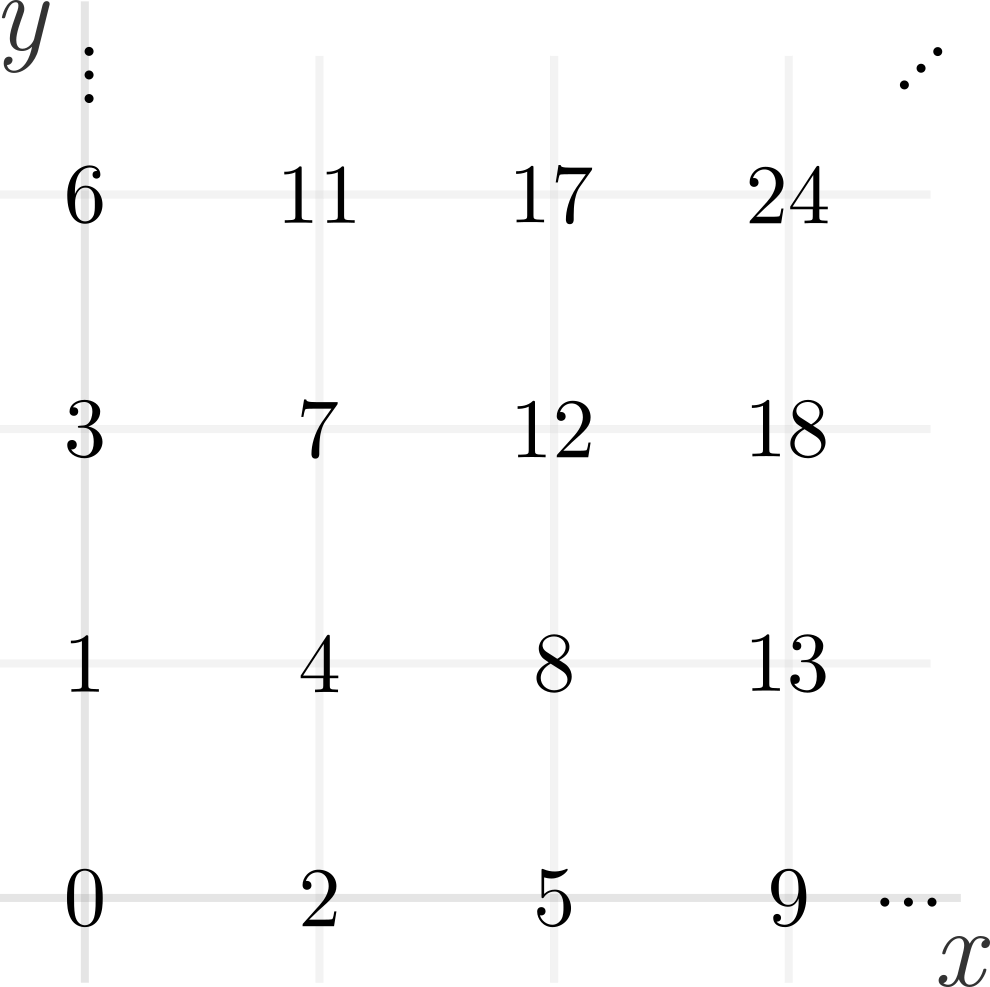
\includegraphics[width=15em]{Immagini/cp.png}
\end{figure}

But also as a "path" taken on the same grid, which traverses each point exactly once:

\begin{figure}[H]
  \centering
  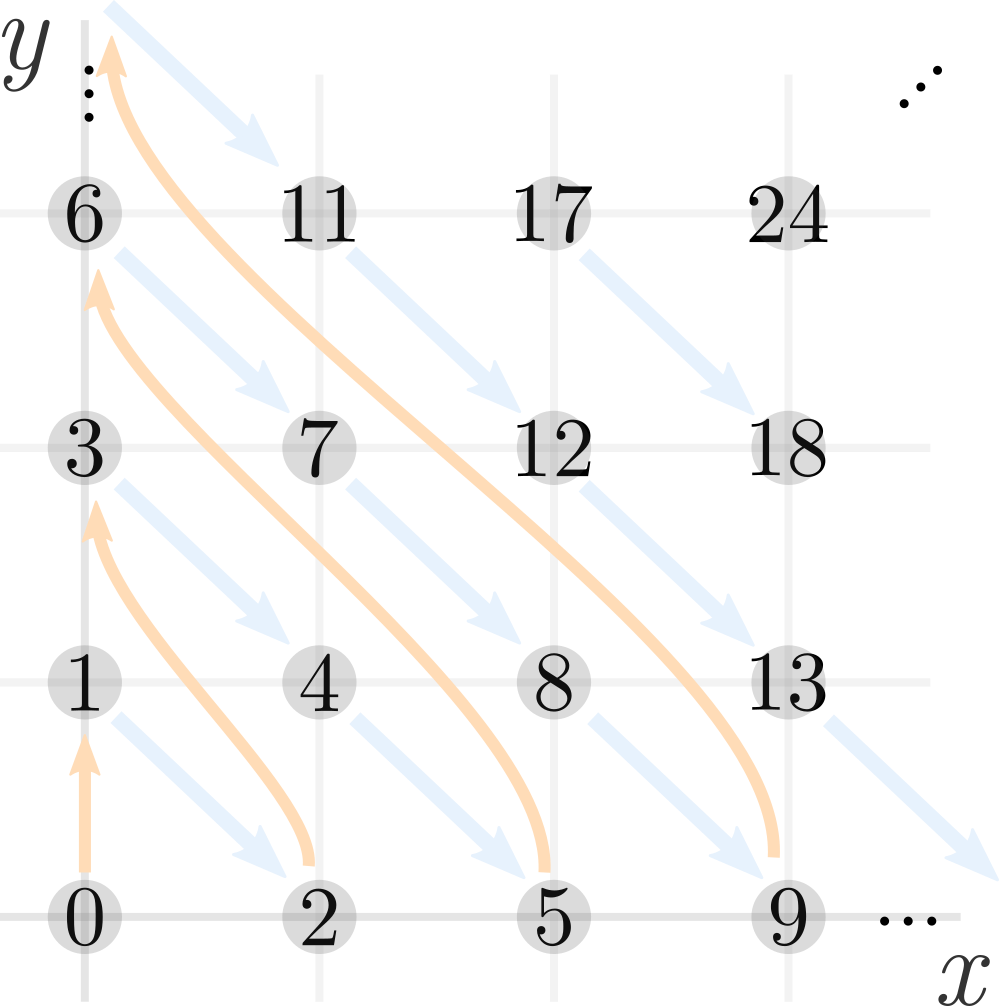
\includegraphics[width=15em]{Immagini/cammino.png}
\end{figure}

Naturally, being bijective means that there exists an inverse function $\rppcu = \big( \rppcu_1, \rppcu_2 \big) : \NN \to \NN^2$,
called the \textbf{Cantor unpairing}, which is usually expressed as
\[ \rppcu(n) = \left( n - \frac{i(1+i)}{2}, \frac{i(3+i)}{2} - n \right) \]
where $i = \left\lfloor \frac{\sqrt{8n + 1} - 1}{2} \right\rfloor $.
We want to implement $\rppcu$ inside $\RPP$, but there's a more natural way to define it than this.

Instead of thinking about $\rppcu$ analytically, let's imagine it again as a path in $\NN^2$:
we start at position $(0, 0)$ and successively apply a series of steps,
moving to $(x+1,y-1)$ if $y > 0$ or to $(0, x+1)$ if $y = 0$.
If we're able to find $\rppcustep \in \RPP$ such that
\[ \rppcustep(x,y) = \begin{cases} (x+1,y-1) &  y > 0 \\
                                   (0, x+1) &   y = 0 \end{cases} \]
then we can define $\rppcui = \rppIt[\rppcustep]$, so that $\rppcui(n, 0, 0)$ applies $n$ steps in the path, and reaches $\big( n, \rppcu_1(n), \rppcu_2(n) \big)$
(the subscript $\mathsf{_{input}}$ is motivated by the fact that we keep the input $n$).

It turns out that it's indeed possible to express $\rppcustep$ in $\RPP$:
\begin{align*}
\rppcustep \ = \ & \rppId_1 \rppPa \rppIf[\rppSu, \rppId_1, \rppId_1] \rppCo \\
                 & \rpprewire{2, 0, 1} \rppCo \\
                 & \rppIf[\rppSu \rppPa \rppPr , \ \rppSu \rppCo \rppSw, \ \rppId_1] \rppCo \\
                 & \rppSw \rppCo \rppIf[\rppPr, \rppId_1, \rppId_1] \rppCo \\
                 & \rppId_1 \rppPa \rppSw
\end{align*}

\makebox[\textwidth][c]{${\small\begin{NiceMatrix}
  \oloch{3-1}{\ y > 0} & x &                                                              & x & \bloch{3-1}{2 \\ 0 \\ 1} & 1 & \bloch{3-1}{\rppIf[\boldsymbol{\rppSu \rppPa \rppPr}, \ \rppSu \rppCo \rppSw, \ \rppId_1]} & 1     & \bloch{2-1}{\rppSw} & x + 1 & \bloch{2-1}{\rppIf[\boldsymbol{\rppPr}, \rppId_1, \rppId_1]} & x + 1 &                     & x + 1 \\
                       & y & \bloch{2-1}{\rppIf[\boldsymbol{\rppSu}, \rppId_1, \rppId_1]} & y &                          & x &                                                                                            & x + 1 &                     & 1     &                                                              & 0     & \bloch{2-1}{\rppSw} & y - 1 \\
                       & 0 &                                                              & 1 &                          & y &                                                                                            & y - 1 &                     & y - 1 &                                                              & y - 1 &                     & 0     \\
\\
  \oloch{3-1}{\ y = 0} & x &                                                              & x & \bloch{3-1}{2 \\ 0 \\ 1} & 0 & \bloch{3-1}{\rppIf[\rppSu \rppPa \rppPr, \ \boldsymbol{\rppSu \rppCo \rppSw}, \ \rppId_1]} & 0     & \bloch{2-1}{\rppSw} & 0     & \bloch{2-1}{\rppIf[\rppPr, \boldsymbol{\rppId_1}, \rppId_1]} & 0     &                     & 0     \\
                       & 0 & \bloch{2-1}{\rppIf[\rppSu, \boldsymbol{\rppId_1}, \rppId_1]} & 0 &                          & x &                                                                                            & 0     &                     & 0     &                                                              & 0     & \bloch{2-1}{\rppSw} & x + 1 \\
                       & 0 &                                                              & 0 &                          & 0 &                                                                                            & x + 1 &                     & x + 1 &                                                              & x + 1 &                     & 0     \\
\\
\end{NiceMatrix}}$}

Notice that we can't directly use $y$ as the condition for the selection $\rppIf$,
because we also want to manipulate $y$ in those calculations.
We get around this limitation by using an ancillary variable initially set to $0$,
which assumes value $1$ or $0$ depending on whether $y>0$ or $y=0$,
and is then set back to $0$ using a variable that we know is positive or equal to zero depending on the case considered.

At this point we can define $\rppcui$ like so:

\noindent\begin{minipage}{.5\linewidth}
\[ \rppcui = \rppIt[\rppcustep] \]
\end{minipage}%
\begin{minipage}{.5\linewidth}
\[\begin{NiceMatrix}
  n & \bloch{4-1}{\rppcui} & n           \\
  0 &                      & \rppcu_1(n) \\
  0 &                      & \rppcu_2(n) \\
  0 &                      & 0           \\
\end{NiceMatrix}\]
\end{minipage}

The function in the other direction is less intricate to define ($\rppcpi$ also keeps the input around, hence the subscript) :

\noindent\begin{minipage}{.5\linewidth}
\[ \rpptr = \rppIt[\rppSu \rppCo \rppinc] \]
\end{minipage}%
\begin{minipage}{.5\linewidth}
\[\begin{NiceMatrix}
  x & \bloch{3-1}{\rpptr} & x \\
  0 &                     & x \\
  0 &                     & \sum_{i=1}^x i \\
\end{NiceMatrix}\]
\end{minipage}

\begin{align*}
  \rppcpi = & \rppinc \rppCo \rppId_1 \rppPa \rpptr \rppCo \\
             & \rppId_1 \rppPa \rppdec \rppCo \rppdec \rppCo \\
             & \rpprewire{0, 3, 1} \rppCo \rppinc \rppCo \rppId_1 \rppPa \rppSw
\end{align*}
\makebox[\textwidth][c]{$\begin{NiceMatrix}
  x & \bloch{2-1}{\rppinc} & x     &                     & x                    &                      & \bloch{2-1}{\rppdec} & x                    & \bloch{4-1}{0\\3\\1} & \bloch{2-1}{\rppinc} &                     & x                        & \Block{4-1}{=} & x           \\
  y &                      & x + y & \bloch{3-1}{\rpptr} & x + y                & \bloch{2-1}{\rppdec} &                      & y                    &                      &                      & \bloch{2-1}{\rppSw} & y                        &                & y           \\
  0 &                      & 0     &                     & x + y                &                      &                      & 0                    &                      &                      &                     & \sum_{i=1}^{x + y} i + x &                & \rppcp(x,y) \\
  0 &                      & 0     &                     & \sum_{i=1}^{x + y} i &                      &                      & \sum_{i=1}^{x + y} i &                      &                      &                     & 0                        &                & 0           \\
\\
\end{NiceMatrix}$}
We can combine $\rppcpi$ and $\rppcui$ to get rid of the input values they both leave behind:
\begin{align*}
\rppcp & = \rppcpi \rppCo \rpprewire{2, 0, 1} \rppCo \rppcui^{-1} \\
\rppcu & = \rppcp^{-1}
\end{align*}
\[\begin{NiceMatrix}
  x & \bloch{4-1}{\rppcpi} & x           & \bloch{3-1}{2\\0\\1} & \rppcp(x,y) & \bloch{4-1}{\rppcui^{-1}} & \rppcp(x,y) \\
  y &                       & y           &                      & x           &                            & 0           \\
  0 &                       & \rppcp(x,y) &                      & y           &                            & 0           \\
  0 &                       & 0           &                      & 0           &                            & 0           \\
\end{NiceMatrix}\]
This is very powerful: we succesfully defined a function which stores data from two positions to just one.
We will discuss pairings at greater lengths in the next paragraphs; for now, let's focus on the technique we used.
In defining the function $\rppcui$ we framed it as a "path" in a two-dimensional grid.
By slightly tweaking $\rppcustep$ we can trace out other paths which helps us solve new problems.

For example, let's imagine starting on coordinates $(0,n)$ and moving each turn in direction $(+1,-1)$ (like before)
but now when we reach $(n,0)$, instead of jumping to $(0,n+1)$ we land again on $(0,n)$, looping in the same diagonal forever:

\begin{figure}[H]
  \centering
  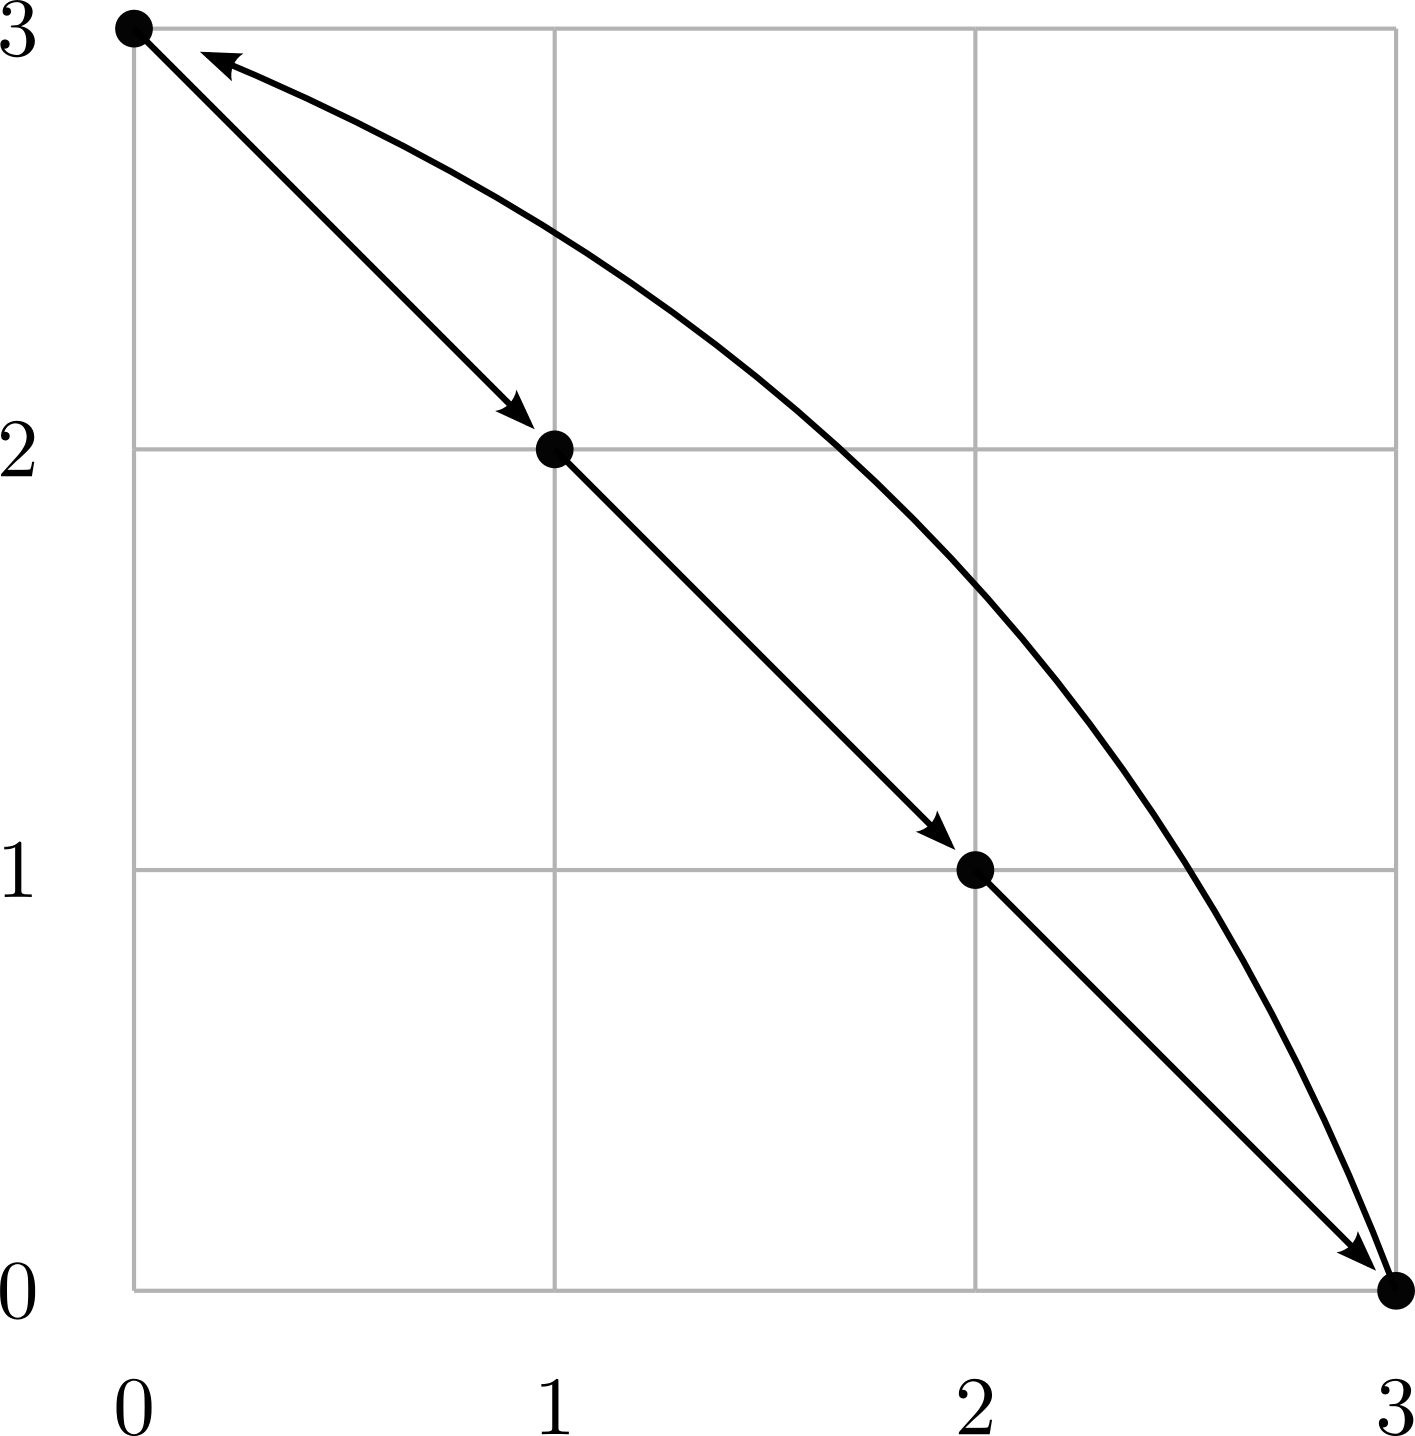
\includegraphics[width=15em]{Immagini/div.png}
\end{figure}

If we call $\rppdivstep$ the function which performs one step of this diagram, by iterating it with $\rppIt[\rppdivstep]$
we've essentially found a way to do modular arithmetic: since it takes $n+1$ steps to get to where we started,
if we perform $m$ steps the $x$ coordinate will be such that $x \equiv m \pmod{n+1}$ and $0 \le x \le n$.
Furthermore, if we increase a counter by one each time we land on $(0,n)$ we can calculate integer division.
The differences between such a $\rppdivstep$ and $\rppcustep$ are minimal (highlighted in bold):

\noindent\begin{minipage}{.5\linewidth}
\begin{align*}
\rppdivstep \ = \ & \rppId_1 \rppPa \rppIf[\rppSu, \rppId_1, \rppId_1] \rppCo \\
                  & \rpprewire{2, 0, 1} \rppCo \\
                  & \rppIf[\rppSu \rppPa \rppPr, \ \boldsymbol{\rppSw \rppPa \rppSu}, \ \rppId_1] \rppCo \\
                  & \rppSw \rppCo \rppIf[\rppPr, \rppId_1, \rppId_1] \rppCo \\
                  & \rppId_1 \rppCo \rppSw \\
\\
\rppdiv =     & \rppIt[\rppdivstep] \\
\end{align*}
\end{minipage}%
\begin{minipage}{.5\linewidth}
\[\begin{NiceMatrix}
  m & \bloch{5-1}{\rppdiv} & m         \\
  0 &                      & r         \\
  n &                      & n + 1 - r \\
  0 &                      & 0         \\
  0 &                      & q         \\
\end{NiceMatrix}\]
\end{minipage}
where $m = q(n + 1) + r$ is the division with remainder of $m$ by $n+1$.

Lastly, there's a way in which we can express the truncated square root function $\left\lfloor \sqrt{n} \right\rfloor$ in $\RPP$.
Of course, the square root is not an invertible function, like division - and like division,
we can get a "remainder" which is the difference $n - \left\lfloor \sqrt{n} \right\rfloor^2$.
We get $\rppsqrtstep$ by tweaking $\rppcustep$ a little - we start off at $(0,0)$ again,
but whenever we reach $(x,0)$ we jump to $(0,x+2)$ and increase a counter by one:

\begin{figure}[H]
  \centering
  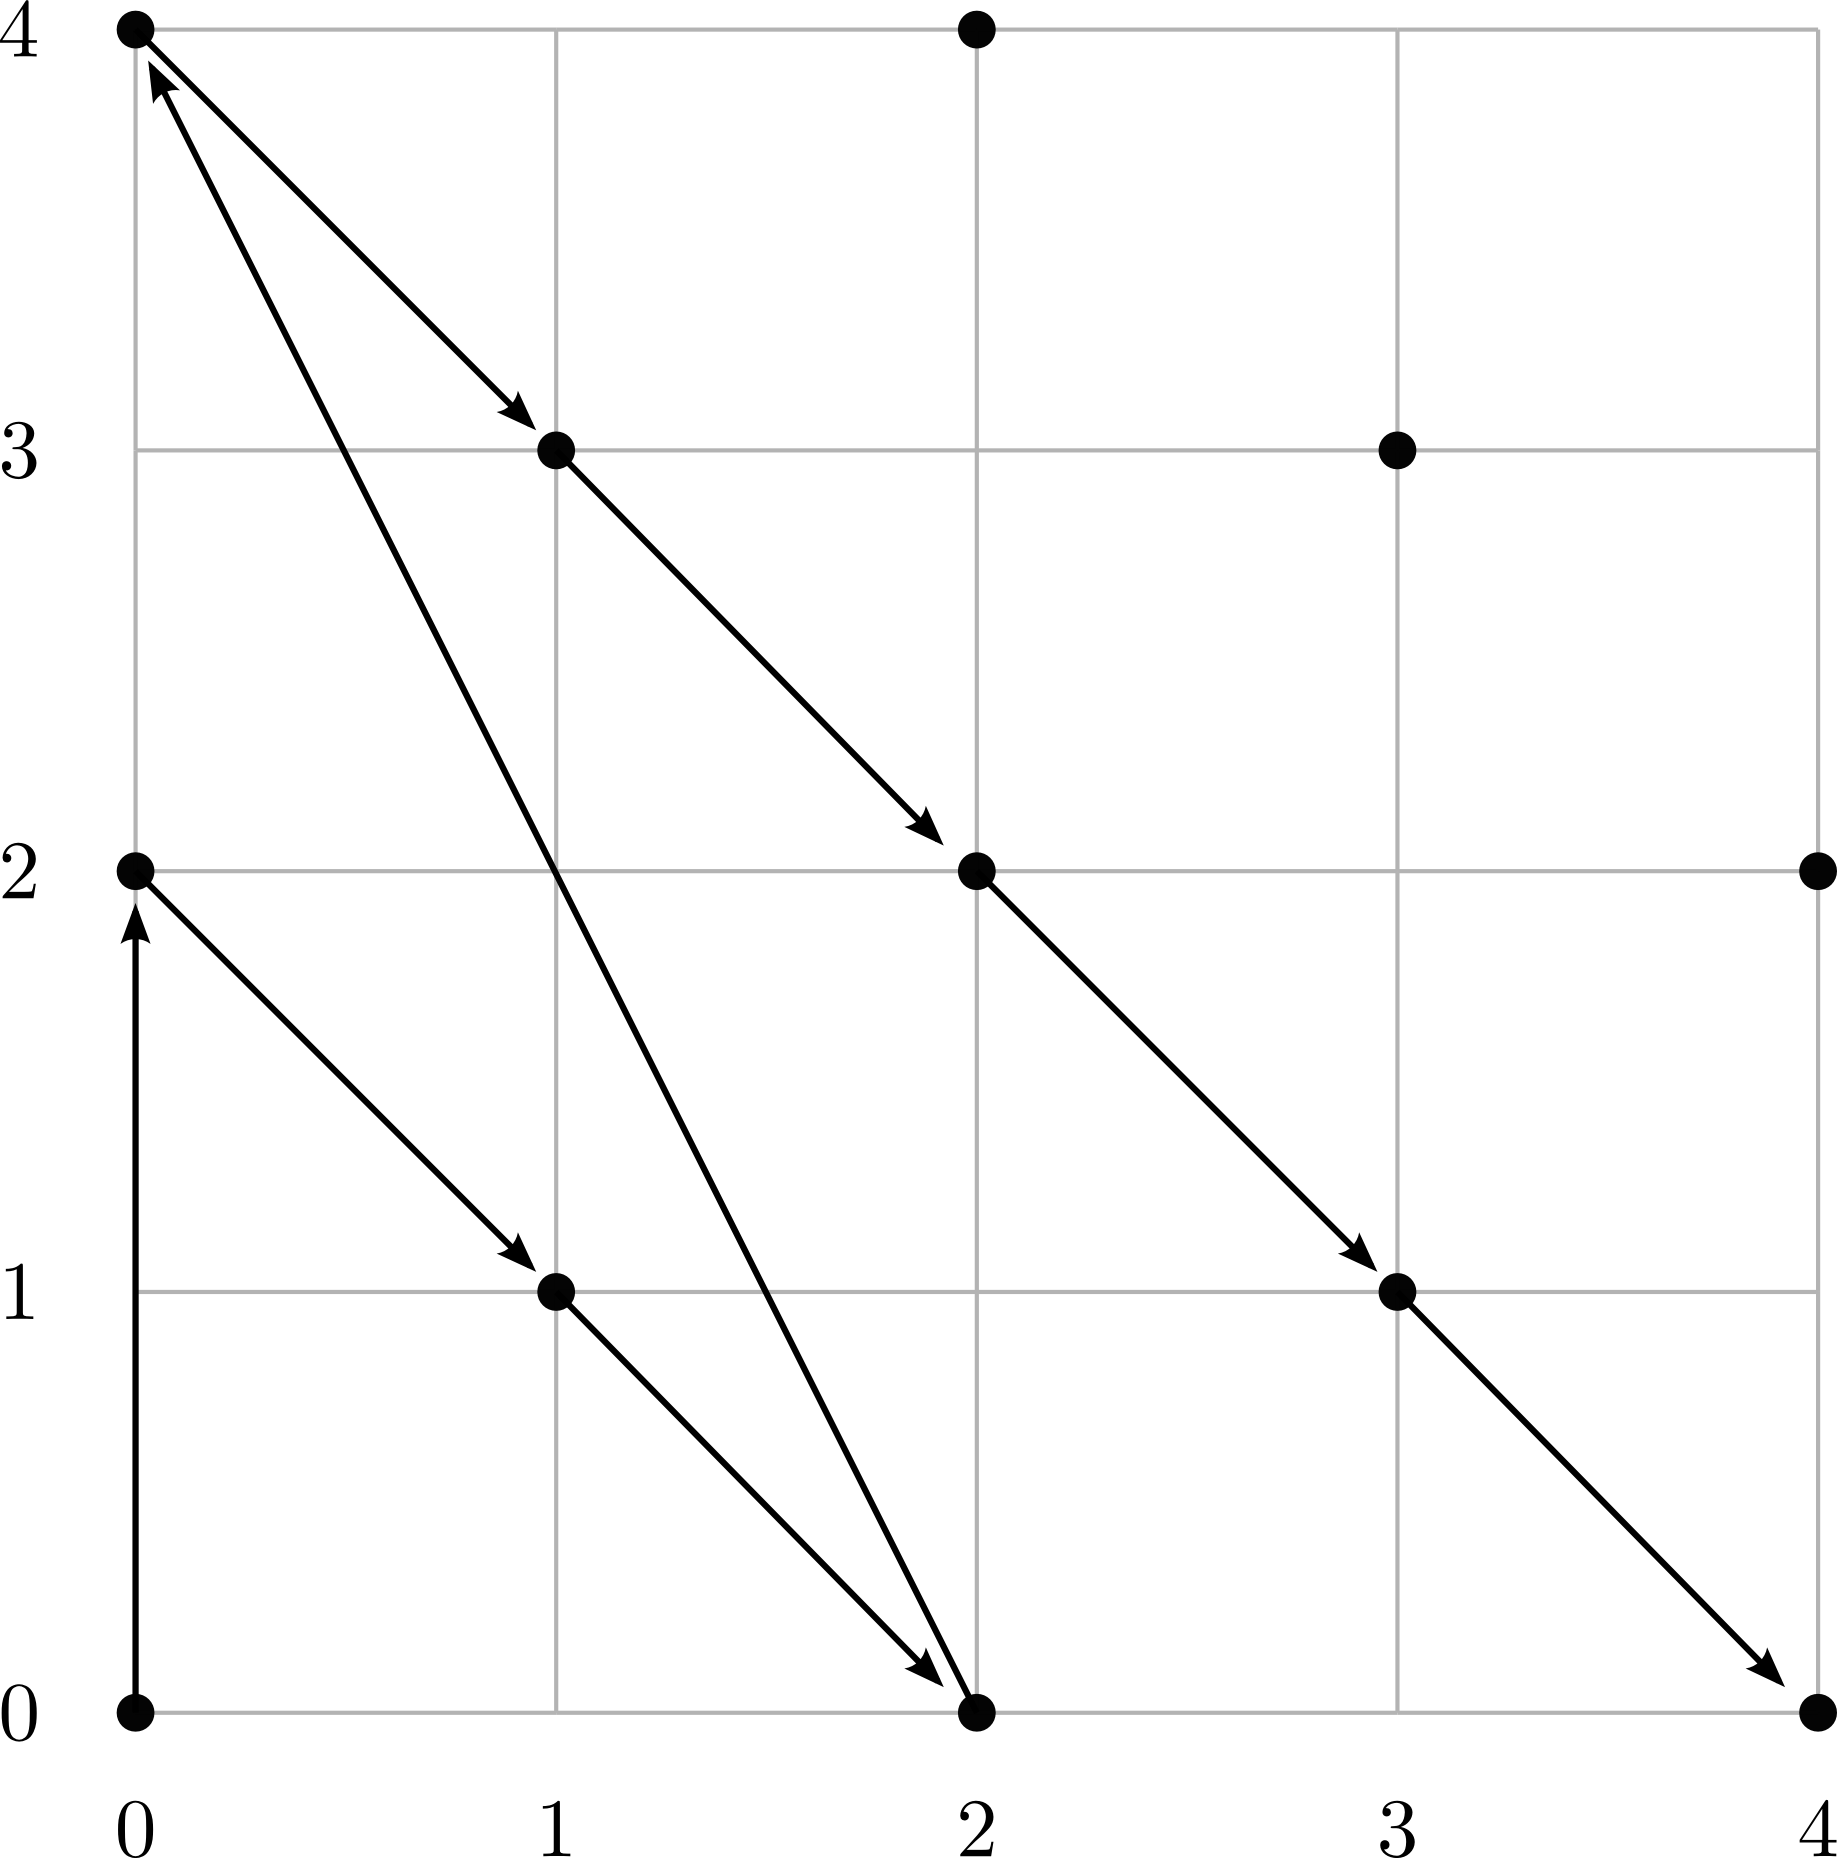
\includegraphics[width=18em]{Immagini/sqrt.png}
\end{figure}

The first jump is performed $1$ step from the starting position $(0,0)$; the next one is performed after $3$ steps, then $5$, $7$ etc.
It's well known that for each $k$, the sum of the first $k$ odd numbers is $1 + 3 + \dots + (2k - 1) = k^2$,
so when we reach the number $k^2$ we've performed $k$ jumps - hence, we calculated a square root (because $k = \sqrt{k^2}$).

Again, we highlight the (minor) differences with $\rppcustep$:

\noindent\begin{minipage}{.5\linewidth}
\begin{align*}
  \rppsqrtstep = & \rppId_1 \rppPa \rppIf[\rppSu, \rppId_1, \rppId_1] \rppCo \\
                 & \rpprewire{2, 0, 1} \rppCo \\
                 & \rppIf[\rppSu \rppPa \rppPr, \ \boldsymbol{\rppSu \rppCo \rppSu \rppCo \rppSw \rppPa \rppSu}, \ \rppId_1] \rppCo \\
                 & \rppSw \rppCo \rppIf[\rppPr, \rppId_1, \rppId_1] \rppCo \\
                 & \rppId_1 \rppCo \rppSw \\
  \\
  \rppsqrt     = & \rppIt[\rppsqrtstep] \\
\end{align*}
\end{minipage}%
\begin{minipage}{.5\linewidth}
\[\begin{NiceMatrix}
  n & \bloch{5-1}{\rppsqrt} & n                      \\
  0 &                       & r                      \\
  0 &                       & 2 \floor{\sqrt{n}} - r \\
  0 &                       & 0                      \\
  0 &                       & \floor{\sqrt{n}}       \\
\end{NiceMatrix}\]
\end{minipage}

where $\floor{\sqrt{n}}$ is the truncated square root and $r = n - \floor{\sqrt{n}}^2$ our "square root remainder".
% The term $2 \floor{\sqrt{n}} - r$ could be cancelled out by adding $r$ and subtracting two times $\floor{\sqrt{n}}$,
% but it'll come in hand soon so we leave it.

\paragraph{Another pairing function}

The Cantor pairing is not the only bijection $\NN^2 \to \NN$.
Another one is $\rppmkpair$ \cite{Carneiro19}, which we will also denote with quotation marks $\gl \cdot, \cdot \gr$:
\[\rppmkpair(x,y) = \gl x,y \gr = \begin{cases} y^2 + x & x < y \\ x^2 + x + y & \text{otherwise} \end{cases} \]
with inverse $\rppunpair = \big( (\cdot)_1, (\cdot)_2 \big) : \NN \to \NN^2$:
\begin{align*}
  \rppunpair(n) = \big( (n)_1, (n)_2 \big) = \begin{cases} \big( n - \floor{\sqrt{n}}^2, \floor{\sqrt{n}} \big)                    & n - \floor{\sqrt{n}}^2 < \floor{\sqrt{n}} \\
                                                           \big( \floor{\sqrt{n}}, n - \floor{\sqrt{n}}^2 - \floor{\sqrt{n}} \big) & \text{otherwise} \end{cases}
\end{align*}

We want to express $\rppmkpair$ as an $\RPP$ function, because we'll need it later.
Similarly to $\rppcp$, we first define functions $\rppmkpairi$, $\rppunpairi$ which keep their original input,
and then combine them to "erase" the inputs and get the true $\rppmkpair$ and $\rppunpair$.

\begin{figure}[H]
  \centering
  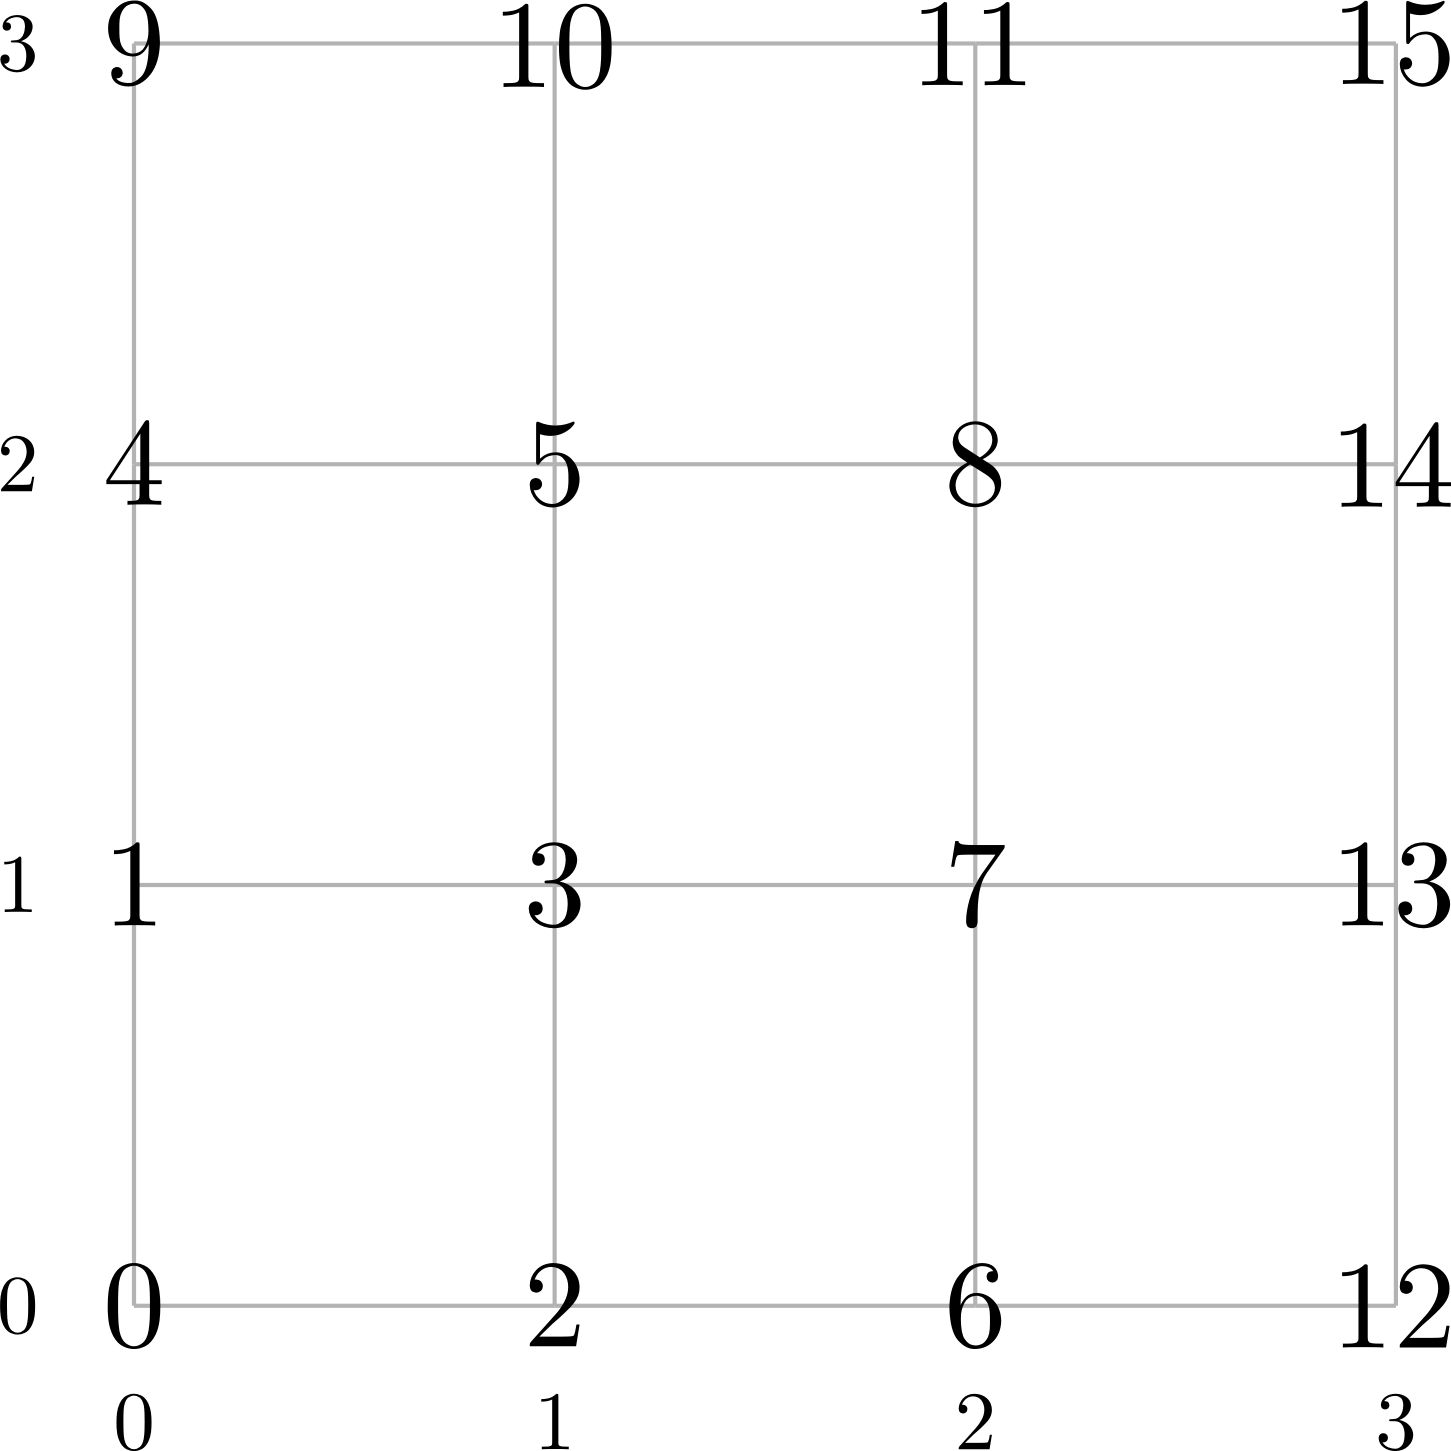
\includegraphics[width=15em]{Immagini/mkpair.png}
\end{figure}

The definitions of $\rppmkpair$ and $\rppunpair$ only involve sums, subtractions, squares, comparisons between naturals and truncated square roots;
we already know how to deal with all of these, so the construction isn't particularly interesting.
For reference, here's the definitions:

\noindent\begin{minipage}{.5\linewidth}
\begin{align*}
\rppmkpairi \ = \ & \rppless \rppCo \\
                   & \rpprewire{2, 0, 1} \rppCo \\
                   & \rppIf[     \rppId_1 \rppPa \rppsquare \rppCo \rppSw \rppCo \rppId_1 \rppPa \rppinc \rppCo \rppSw, \\
                   & \hspace{1em}\rppId_1 \rppPa \rppinc \rppCo \rppSw \rppCo \rppId_1 \rppPa (\rppsquare \rppCo \rppinc) \rppCo \rppSw, \\
                   & \hspace{1em}\rppId_1] \rppCo \\
                   & \rpprewire{1, 2, 0} \rppCo \\
                   & \rppless^{-1} \\
\end{align*}
\end{minipage}%
\begin{minipage}{.5\linewidth}
\[\begin{NiceMatrix}
  n & \bloch{5-1}{\rppmkpairi} & n                \\
  m &                           & m                \\
  0 &                           & 0                \\
  0 &                           & \gl n, m \gr \\
  0 &                           & 0                \\
\end{NiceMatrix}\]
\end{minipage}

\noindent\begin{minipage}{.5\linewidth}
\begin{align*}
\rppunpairifwd \ = \  & \rppsqrt \rppCo \\
                                   & \rpprewire{0, 1, 4, 2, 3} \rppCo \\
                                   & \rppId_2 \rppPa \rppdec \rppCo \\
                                   & \rppId_3 \rppPa \rppNe \rppCo \\
                                   & \rppId_3 \rppPa \rppIf[\rppId_1, \rppId_1, \rppPr] \rppCo \\
                                   & \rpprewire{0, 4, 1, 2, 3} \\
\end{align*}
\end{minipage}%
\begin{minipage}{.5\linewidth}
\[\begin{NiceMatrix}
  n & \bloch{5-1}{\rppunpairifwd} & n                                         \\
  0 &                             & s                                         \\
  0 &                             & n - \floor{\sqrt{n}}^2                    \\
  0 &                             & \floor{\sqrt{n}}                          \\
  0 &                             & n - \floor{\sqrt{n}}^2 - \floor{\sqrt{n}} \\
\end{NiceMatrix}\]
\end{minipage}

where $s = -1 \ $ if $ \ n - \floor{\sqrt{n}}^2 < \floor{\sqrt{n}}$, and $s = 0$ otherwise.

\noindent\begin{minipage}{.5\linewidth}
\begin{align*}
\rppunpairi \ = \ & \rppunpairifwd \\
                   & \rppId_1 \rppPa \rppIf \big[ \rppId_1, \\
                   & \hspace{2.6em}         \rpprewire{0, 1, 3, 2, 4} \rppCo \rppId_1 \rppPa \rppinc \rppPa \rppinc \rppCo \rpprewire{0, 1, 3, 2, 4}, \\
                   & \hspace{2.6em}         \rpprewire{0, 3, 1, 4, 2} \rppCo \rppinc \rppPa \rppinc \rppCo \rpprewire{0, 2, 4, 1, 3} \big] \rppCo \\
                   & \rppunpairifwd^{-1} \\
\end{align*}
\end{minipage}%
\begin{minipage}{.5\linewidth}
\[\begin{NiceMatrix}
  n & \bloch{7-1}{\rppunpairi} & n               \\
  0 &                          & 0               \\
  0 &                          & 0               \\
  0 &                          & 0               \\
  0 &                          & 0               \\
  0 &                          & (n)_1 \\
  0 &                          & (n)_2 \\
\end{NiceMatrix}\]
\end{minipage}

\noindent\begin{minipage}{.5\linewidth}
\begin{align*}
\rppmkpair \ = \ & \rppmkpairi \rppCo \rpprewire{3, 2, 4, 5, 6, 0, 1} \rppCo \rppunpairi^{-1} \\
\rppunpair \ = \ & \rppmkpair^{-1} \\
\end{align*}
\end{minipage}%
\begin{minipage}{.5\linewidth}
\[\begin{NiceMatrix}
  n & \bloch{7-1}{\rppmkpair} & \gl n, m \gr \\
  m &                         & 0                \\
  0 &                         & 0                \\
  0 &                         & 0                \\
  0 &                         & 0                \\
  0 &                         & 0                \\
  0 &                         & 0                \\
\end{NiceMatrix}\]
\end{minipage}

With $\rppunpairi$ we make use of \textit{Bennet's trick} \cite{perumalla2013chc}:
we perform a computation $\rppunpairifwd$ which gives us the result we need, alongside some other useless data.
The obvious next step would be to throw away the useless data and just keep the result,
but in reversible computing we can't erase information.
Instead, we store the result and then run the whole computation backwards:
in this way, we get to where we started but with our result.

In general, reversible programs must always face the following problem: how to best manage information?
Where do we put things we don't need?
This is something we'll have to think about when we analyze $\PRF$-completeness,
and pairing functions will be the key.

\paragraph*{Verifying the behaviour}

We've looked at some functions which can be defined within $\RPP$.
Using Lean we can input the definitions and then test them in a concrete way,
to check if they work correctly:
\begin{lstlisting}
#eval ‹square› [22, 0, 0]  -- [22, 484, 0]
#eval ‹square› [6, 100, 0] -- [6, 136, 0]
                              -- seems fine, I guess
\end{lstlisting}
But we can do much more: we can \textit{prove} that they work correctly,
in the same environment where we defined them.

This is a big step over defining them in a standard programming language and then
writing a proof of their correctness on "pen and paper",
because in that case there's no guarantee that what has been defined on machine
is the same thing as what is being discussed in the proof:
they're two different objects living in different worlds,
linked only by our commitment to avoid mistakes in any of the two.

Instead, in Lean we can define \lstinline{square} and then write on the following line
\begin{lstlisting}
@[simp] lemma square_def (n : ℕ) (x : ℤ) (X : list ℤ) :
  ‹square› (n :: x :: 0 :: X) = n :: (x + n * n) :: 0 :: X :=
by simp [square, ev]
\end{lstlisting}
and if there's a typo in the definition, or a hole in the argumentation,
the proof will just fail.

Even better: if \lstinline{square} is used in the definition of other functions,
like \lstinline{mkpairᵢ}, when we verify the correctness of \lstinline{mkpairᵢ}
we'll already have the theorem about \lstinline{square} at our disposal.

As an example let's see some of these theorems:
\begin{lstlisting}
@[simp] lemma inc_def (n : ℕ) (x : ℤ) (X : list ℤ) :
  ‹inc› (n :: x :: X) = n :: (x + n) :: X :=
begin
  rw [inc], simp [ev],
  -- ring is used to solve automatically simple equations 
  induction n generalizing x, simp, simp [ev, *], ring
end
\end{lstlisting}
The proof is by induction on \lstinline{n} and it's nothing remarkable.
What's interesting is that we mark this lemma as \lstinline{@[simp]}.
The next proof is about \lstinline{dec := inc⁻¹}:
\begin{lstlisting}
lemma dec_def (n : ℕ) (x : ℤ) (X : list ℤ) :
  ‹dec› (n :: x :: X) = n :: (x - n) :: X :=
begin
  -- ⊢ ‹dec› (n :: x :: X) = n :: (x - n) :: X
  rw dec,
  -- ⊢ ‹inc⁻¹› (n :: x :: X) = n :: (x - n) :: X
  rw inv_iff,
  -- ⊢ ‹inc› (n :: (x - n) :: X) = n :: x :: X
  rw inc_def,
  -- ⊢ n :: (x - n + n) :: X = n :: x :: X
  simp,
  -- goals accomplished
end
\end{lstlisting}
We made good use of our lemma \lstinline{inc_def}.
However, since we marked it as \lstinline{simp}, the proof can be greatly shortened:
\begin{lstlisting}
@[simp] lemma dec_def (n : ℕ) (x : ℤ) (X : list ℤ) :
  ‹dec› (n :: x :: X) = n :: (x - n) :: X :=
by simp[dec]
\end{lstlisting}
and in turn we mark \lstinline{dec_def} as \lstinline{@[simp]},
commencing our snowball of automation.

Indeed, each one of these theorems can be proven with (relatively) little effort
by first setting things up right and then unleashing the simplifier.
As an example, here's \lstinline{sqrt_def}:
\begin{lstlisting}
@[simp] lemma sqrt_def (n : ℕ) (X : list ℤ) :
  ‹sqrt› (n :: 0 :: 0 :: 0 :: 0 :: X) =
  n :: (n - √n * √n) :: (√n + √n - (n - √n * √n))
    :: 0 :: √n :: X :=
begin
  -- initial set up
  simp [sqrt, ev],
  induction n with n hn,
  simp,
  rw [function.iterate_succ_apply', hn], clear hn,

  -- divides the proof in two cases
  cases (sqrt_succ_or n) with h h,

  -- first case
  -- the tactic have introduces a new goal
  -- which is added to the hypotheses once solved
  have H₁ := sqrt_lemma_1 n h,
  have H₂ : (0 : ℤ) < n - √n * √n + 1,
    by { have h := nat.sqrt_le n, norm_cast, linarith },
  simp[sqrt_step, ev, rewire, *], split, ring, ring,

  -- second case
  have H₁ := sqrt_lemma_2 n h,
  have H₂ : (n : ℤ) = √n + √n + √n * √n,
    by { symmetry, rw ←sub_eq_zero, rw ←H₁, ring },
  simp[sqrt_step, ev, rewire, *], split, ring, ring
end
\end{lstlisting}
There's an initial set up, then it splits into two cases.
In each, some hypothesis are added to aid \lstinline{simp} and \lstinline{ring},
which are subsequently called to finish the job.

Since we're interested in using the simplifier as much as possible,
we've been careful stating our theorems.
Another way to express \lstinline{inc_def} would've been
\begin{lstlisting}
@[simp] lemma inc_def (n : ℕ) (x : ℤ) (X : list ℤ) :
  ‹inc› [n, x] = [n, x + n]
\end{lstlisting}
but this can be applied only when the input list is of length exactly 2;
often we have something like \lstinline{‹inc› (n :: x ::X)} with \lstinline{X : list ℤ}.
By theorem \lstinline{ev_split} we know that
\begin{lstlisting}
‹inc› (n :: x :: X) = ‹inc› [n, x] ++ X
\end{lstlisting}
but remember that we can't mark \lstinline{ev_split} as \lstinline{@[simp]} because
that would lead to infinite loops.
Thus, that formulation of the properties of \lstinline{inc} is not very \lstinline{simp}-friendly.
By framing \lstinline{inc_def} as we did, this problem disappears.

We restate that the purpose of Lean is not being an automatic theorem prover.
However, it's nice when it can be used in that way.

\section{PRF-completeness} \label{prfcompleteness}

We've just seen that the class of functions $\RPP$ is not quite as limited as it might seem at first sight,
containing things like square roots and pairings.
At this point we could ask ourselves - what exactly \textit{can} (or can't) we express in $\RPP$?
Given a function, is there a quick way to tell if it's possible to include it in $\RPP$ or not?

The answer is yes - in fact, $\RPP$ were created already with this question in mind.
Specifically, they can be thought of as the reversible counterpart to another,
more famous class of function: the \textit{Primitive Recursive Functions} \cite{odifreddi1989book}.

\begin{definition}[Primitive Recursive Functions]
The class of \textbf{Primitive Recursive Functions} is the smallest subset of function $\NN^n \to \NN$ satisfying the following conditions:
\begin{itemize}
\item The \textbf{constant function} $\prZero(x) = 0$ belongs to $\PRF$.
\item The \textbf{successor function} $\prSucc(x) = x+1$ belongs to $\PRF$.
\item The $n$-ary \textbf{projection function} $\prProj{n}{i}(x_1, \dots, x_n) = x_i$ belongs to $\PRF$
for all $n \in \NN$ and $1 \le i \le n$.
\item If $F_1, \dots, F_m : \NN^n \to \NN$ and $G : \NN^m \to \NN$ belong to $\PRF$,
then the \textbf{composition} $G \big( F_1(\boldsymbol{x}), \dots, F_m(\boldsymbol{x}) \big)$ belongs to $\PRF$.
\item If $F:\NN^n \to \NN$ and $G:\NN^{n+2} \to \NN$ belong to $\PRF$,
then the function obtained by \textbf{primitive recursion} $H:\NN^{n+1} \to \NN$ such that
\begin{align*}
  H(\boldsymbol{x}, 0)   = & F(\boldsymbol{x}) \\
  H(\boldsymbol{x}, y+1) = & G \big( \boldsymbol{x}, y, h(\boldsymbol{x}, y) \big)
\end{align*}
belongs to $\PRF$.
\end{itemize}
\end{definition}

Primitive recursion is a way to express iteration on the variable $y$,
in a way somewhat similar to the \lstinline{Nat} induction principle \lstinline{Nat.rec} present in Lean:
if we've defined $z=H(\boldsymbol{x},y)$ then we can define $H(\boldsymbol{x},y+1)$ as $G(\boldsymbol{x},y,z)$,
which is something that only depends on the parameter $\boldsymbol{x}$, the iterator $y$ and the previously calculated value $z$.

The importance of this class of functions lies in the simplicity of the definition,
and the fact that most commonly used functions $\NN^n \to \NN$ belong to $\PRF$.

For example here's our good friend $\pradd : \NN^2 \to \NN$:
\begin{align*}
  \pradd(x, 0)   = & \prProj{1}{1}(x) = x \\
  \pradd(x, y+1) = & \prSucc \big( \prProj{3}{3} \big( x,y,\pradd(x,y) \big) \big) = \prSucc(\pradd(x,y)) = \pradd(x,y)+1
\end{align*}
which is obtained by primitive recursion using $\prProj{1}{1}$ and $\prSucc \circ \prProj{3}{3}$.

Primitive recursive functions are a thoroughly studied object and we know many facts about them.
For example, not all functions are primitive recursive, even if those functions are effectively computable:
an example is given by the Ackermann function
\begin{align*}
  \prack(0, n)     \ = \ & n + 1 \\
  \prack(m+1, 0)   \ = \ & \prack(m, 1) \\
  \prack(m+1, n+1) \ = \ & \prack(m, \prack(m+1,n))
\end{align*}
We know that this can't possibly belong to $\PRF$ because there's a limit on how rapidly primitive recursive functions can grow,
and $\prack$ exceeds this limit.
Even small inputs lead to enormous outputs - for example, $\prack(4,2) = 2^{65536}-3$.

Here we delineate the relationship between $\PRF$ and $\RPP$:

\begin{theorem}[$\PRF$-completeness] \label{prftheorem}
Let $F : \NN^k \to \NN$ belong to $\PRF$.
Then, there exists $a \in \NN$ and $f : \ZZ^{1+k+a} \to \ZZ^{1+k+a}$ in $\RPP$ such that for all $z \in \ZZ$ and $\boldsymbol{x} \in \NN^k$,
\[\begin{NiceMatrix}[nullify-dots]
  z              & \bloch{3-1}{f} & z + F(\boldsymbol{x}) \\
  \boldsymbol{x} &                & \boldsymbol{x}        \\
  \boldsymbol{0} &                & \boldsymbol{0}        \\
\end{NiceMatrix}\]
where $\boldsymbol{0} = (0, \dots, 0)$ is a tuple of length $a$.
\end{theorem}

\begin{claim}[$\PRF$-soundness] \label{prfclaim}
Every $f \in \RPP$ has a representative inside $\PRF$ obtainable via the bijection which exists between $\ZZ$ and $\NN$.
\end{claim}

These two statements together mean that, in a sense, $\RPP$ and $\PRF$ are equivalent:
anything expressible in $\PRF$ can also be encoded in $\RPP$ and vice versa.
So, no matter how hard we try, we'll never be able to implement something like $\prack$ in $\RPP$.

Theorem \ref{prftheorem} has been succesfully verified in Lean (and also Coq): we will focus on this in the following paragraph.
On the other hand, claim \ref{prfclaim} is intuitively true for those familiar with $\PRF$ functions
and annoying to write down precisely, so for the moment no energies have been spent in trying to formalize it in a proof assistant.

\paragraph{$\PRF$-completeness in Lean}

As usual, there's more than one way in which our result can be proven.
We could come up with our definition of $\PRF$ in Lean,
but actually in Mathlib there's already one present.
By stating our theorem in terms of the already-defined $\PRF$,
we "link" our object ($\RPP$ functions) with already established ones;
building on top of what has already been done is both convenient and effective.

Truth to be told, there are at least two notions of $\PRF$ in Mathlib \cite{Carneiro19}.
First the one that most closely resembles the definition we've given:
\begin{lstlisting}
inductive primrec' : ∀ {n}, (vector ℕ n → ℕ) → Prop
| zero : @primrec' 0 (λ _, 0)
| succ : @primrec' 1 (λ v, succ v.head)
| nth {n} (i : fin n) : primrec' (λ v, v.nth i)
| comp {m n f} (g : fin n → vector ℕ m → ℕ) :
  primrec' f → (∀ i, primrec' (g i)) →
  primrec' (λ a, f (of_fn (λ i, g i a)))
| prec {n f g} : @primrec' n f → @primrec' (n+2) g →
  primrec' (λ v : vector ℕ (n+1),
    v.head.elim (f v.tail) (λ y IH, g (y ::ᵥ IH ::ᵥ v.tail)))
\end{lstlisting}
Notice the type: it's a function that takes as inputs a number \lstinline{n : ℕ},
a function \lstinline{vector ℕ n → ℕ} and returns a proposition \lstinline{Prop} -
in short, it's an \textbf{inductive proposition}.\footnote{We could've used the same approach with $\RPP$, inductively defining the proposition
"this is a reversible primitive permutation". We haven't explored this alternative.}
The meaning of this, is that we're defining inductively the statement "this is a primitive recursive function".
For example, the third base case \lstinline{nth} tells us that the function \lstinline{(λ v, v.nth i)}
which given a vector \lstinline{v} returns its \lstinline{i}-th element, is a primitive recursive function.
This is stated by the fact \lstinline{primrec' (λ v, v.nth i)}, which is a proposition.
The last case \lstinline{prec} takes as input the statements that functions \lstinline{f} and \lstinline{g} are primitive recursive,
and declares that a more complicated function (given by primitive recursion of \lstinline{f} and \lstinline{g}) is also primitive recursive.

Even if \lstinline{primrec'} matches our notion of $\PRF$, it's pretty complicated.
Its power makes it a good definition if we want to prove that something is a primitive recursive function,
but a bad one if instead we want to show a result about $\PRF$.
For that, it's better to use another definition:
\begin{lstlisting}
inductive primrec : (ℕ → ℕ) → Prop
| zero : primrec (λ n, 0)
| succ : primrec succ
| left : primrec (λ n, n.unpair.1)
| right : primrec (λ n, n.unpair.2)
| pair {f g} : primrec f → primrec g →
   primrec (λ n, mkpair (f n) (g n))
| comp {f g} : primrec f → primrec g → primrec (λ n, f (g n))
| prec {f g} : primrec f → primrec g →
   primrec (unpaired (λ z n, n.elim (f z)
    (λ (y IH : ℕ), g (nat.mkpair z (nat.mkpair y IH)))
    n))
\end{lstlisting}
At first sight, this looks like something totally different.
It's still an inductive proposition, but takes as argument just unary functions \lstinline{ℕ → ℕ}, not of arbitrary arity.
The first two cases \lstinline{zero} and \lstinline{succ} are straightforward but the third and fourth are somewhat alien -
investigating further, we discover that \lstinline{unpair} is the $\rppunpair$ function introduced in the previous section!
It's also present \lstinline{mkpair}, not only in the base case \lstinline{pair} but also in the primitive recursive case \lstinline{prec}.
What's going on is that we use pairing functions to work with functions \lstinline{ℕ → ℕ} instead of \lstinline{n}-ary ones.
Composition becomes a lot easier, and to express functions with higher arity we use \lstinline{pair} to "join" two values,
which can then be retrieved using the functions \lstinline{left} and \lstinline{right}.

The definition \lstinline{primrec} might seem weird, but to be honest, that's not something we have to worry about:
in Mathlib it's already proven that \lstinline{primrec} and \lstinline{primrec'} are equivalent definitions - meaning,
every \lstinline{primrec} is \lstinline{primrec'},
and there's a certain sense in which every \lstinline{primrec'} can be encoded as a \lstinline{primrec}.

At this point the choice is obvious: we have to prove that all $\PRF$ are expressable as $\RPP$,
and showing that using \lstinline{primrec} is much simpler than with \lstinline{primrec'}.
To state the theorem we first define the proposition \lstinline{encode F f} which means
"\lstinline{F : ℕ → ℕ} can be encoded in \lstinline{RPP} through \lstinline{f}":
\begin{lstlisting}
def encode (F : ℕ → ℕ) (f : RPP) := ∀ (z : ℤ) (n : ℕ),
  ‹f› (z :: n :: repeat 0 (f.arity-2)) =
      (z + F n) :: n :: repeat 0 (f.arity-2)
\end{lstlisting}
Our main thesis becomes
\begin{lstlisting}
theorem completeness (F : ℕ → ℕ) :
  nat.primrec F → ∃ f : RPP, encode F f
\end{lstlisting}
that is: for all \lstinline{F : ℕ → ℕ} such that \lstinline{primrec F},
there exists \lstinline{f : RPP} which encode \lstinline{F}.

To show this result we proceed by induction on the proposition \lstinline{nat.primrec F},
generating 7 goals (one for each case in the definition of \lstinline{primrec}).
Let's see the second one, involving \lstinline{primrec.succ}:
\begin{lstlisting}
  case nat.primrec.succ
  ⊢ ∃ (f : RPP), encode nat.succ f
\end{lstlisting}
By definition of \lstinline{encode},
this means we have to find an \lstinline{f : RPP} such that
\begin{lstlisting}
‹f› (z :: n :: repeat 0 (f.arity - 2)) =
(z + n.succ) :: n :: repeat 0 (f.arity - 2)
\end{lstlisting}
Our candidate is \lstinline{succ := Su ;; Sw ;; inc ;; Sw}, which has the following behaviour:
\begin{lstlisting}
lemma succ_def (z : ℤ) (n : ℕ) :
  ‹succ› [z, n] = [z + n.succ, n] :=
by { simp [succ, ev], ring }
\end{lstlisting}
which is just another way to rephrase \lstinline{encode nat.succ succ}.
To present a witness of an existential proposition we use the tactics \lstinline{use}:
\begin{lstlisting}
-- ⊢ ∃ (f : RPP), encode nat.succ f
use succ,
-- ⊢ encode nat.succ succ
exact succ_def,
-- goals accomplished
\end{lstlisting}

We proceed like this for each case:
we construct a suitable function \lstinline{f : RPP}
and then prove \lstinline{encode F f} for the given \lstinline{F}.
For the base cases this is something very simple; for the inductive cases more care is needed.

To illustrate this, here's the case \lstinline{primrec.comp}:
\begin{lstlisting}
  G₁, G₂ : ℕ → ℕ
  h₁ : nat.primrec G₁
  h₂ : nat.primrec G₂
  ih₁ : ∃ (f : RPP), encode G₁ f
  ih₂ : ∃ (f : RPP), encode G₂ f
  ⊢ ∃ (f : RPP), encode (λ (n : ℕ), G₁ (G₂ n)) f
\end{lstlisting}
We will ultimately solve this by proposing as witness the function \lstinline{pair f g : RPP},
and then proving it's the right one through the lemma \lstinline{pair_def}.
To guarantee its correct behaviour, the inductive hypotheses \lstinline{ih₁} and \lstinline{ih₂} are crucial.
Let's study the first one: \lstinline{ih₁} can be broken down using the \lstinline{cases} tactics,
giving us the hypothesis
\begin{lstlisting}
g₁ : RPP
ih₁ : encode G₁ g₁
\end{lstlisting}
which means
\begin{lstlisting}
‹g₁› (z :: n :: repeat 0 (g₁.arity - 2)) =
(z + G₁ n) :: n :: repeat 0 (g₁.arity - 2)
\end{lstlisting}
The problem with this hypothesis is that it requires us
to have exactly \lstinline{g₁.arity - 2} trailing zeroes,
so if there's actually more than that, \lstinline{simp} can't use the hypothesis.
To solve this we strengthen our hypothesis to \lstinline{encode_le G₁ g₁}
which works for any number of trailing zeroes greater than \lstinline{g₁.arity - 2}:
\begin{lstlisting}
-- encode_le G₁ g₁:
∀ (a : ℕ), f.arity-2 ≤ a →
‹g₁› (z :: n :: repeat 0 a) =
(z + G₁ n) :: n :: repeat 0 a)
\end{lstlisting}
Actually, \lstinline{encode_le} is a lemma that states precisely
the fact that we can indeed strenghten our hypotheses like this.

We've solved a problem but created another one:
usually in the goal the trailing zeroes look something like
\begin{lstlisting}
-- pair_fwd f g is an auxiliary function
-- used in the definition of pair 
repeat 0 ((pair_fwd f g).arity - 3)
\end{lstlisting}
and so to use \lstinline{encode_le G₁ g₁} we need to make sure that
that number of zeroes is larger than \lstinline{f.arity-2}, i.e.
\begin{lstlisting}
f.arity-2 ≤ (pair_fwd f g).arity - 3
\end{lstlisting}
For this reason, we first prove a lemma which controls
the arity of \lstinline{pair_fwd f g}:
\begin{lstlisting}
lemma pair_fwd_arity (f g : RPP) : ∃ a,
  (pair_fwd f g).arity = a + 7 ∧
  f.arity-2 ≤ a + 4 ∧
  g.arity-2 ≤ a + 3
\end{lstlisting}
which is stated in an odd way using existentials to make it more \lstinline{simp}-friendly.
After these preparations, the proof of \lstinline{pair_fwd_def}
(and of \lstinline{pair_def}) consists of nothing more than
an initial setup and then a call to the simplifier.

\paragraph{}

The most complicated - and the most interesting - case is the last one,
about primitive recursion.
Let's look at the definition again:
\begin{lstlisting}
prec {f g} : primrec f → primrec g →
  primrec (unpaired (λ z n, n.elim (f z)
    (λ (y IH : N), g (nat.mkpair z (nat.mkpair y IH)))
    n))
\end{lstlisting}
Given $F, G \in \PRF$ let's call $H$ the function given by \lstinline{primrec.prec}
(which isn't just standard primitive recursion!).
Let $\gl x, y \gr = \rppmkpair(x,y)$ and $\big( (n)_1, (n)_2 \big) = \rppunpair(n)$,
then $H$ is given by
\[ H(x) = \prPrec[F,G]\big( (x)_1, (x)_2 \big) \]
where we define $\prPrec[F,G] : \NN^2 \to \NN$ as
\begin{align*}
  \prPrec[F,G](z,0) \ = \ & F(z) \\
  \prPrec[F,G](z, n+1) \ = \ & G \big( \gl z, \gl n, \prPrec[F,G](z,n) \gr \gr \big)
\end{align*}

Let's assume that $f, g \in \RPP$ encode respectively $F, G \in \PRF$, i.e.
$f(z, n, \boldsymbol{0}) = (z+F(n), n, \boldsymbol{0})$ and $g(z, n, \boldsymbol{0}) = (z+G(n), n, \boldsymbol{0})$.
Then, we simulate a single iteration of $\prPrec[F,G]$ by $\rppprecstep[g] \in \RPP$ given by

\begin{align*}
\rppprecstep[g] \ = \ & \rppId_2 \rppPa \rppmkpair \rppCo                               \\
                      & \rppId_1 \rppPa \rppmkpair \rppCo                               \\
                      & \rppId_1 \rppPa (\rppSw \rppCo g) \rppCo                        \\
                      & \rppId_2 \rppPa \rppunpair \rppCo                               \\
                      & \rppId_3 \rppPa \rppunpair \rppCo                               \\
                      & \rpprewire{2, 3, 1, 0, 4} \rppCo                                \\
                      & \rppId_1 \rppPa \rppSu \rppPa \rppId_1 \rppPa \rppmkpair \rppCo \\
                      & \rpprewire{3, 0, 1, 2}                                          \\
\end{align*}

Below is a diagram showing each step of the computations of $\rppprecstep[g]$.
The variables $s, s' \in \NN$ are "junk" whose values we don't care about.

\makebox[\textwidth][c]{\begin{NiceMatrixBlock}
$\begin{array}{c}
\begin{NiceMatrix}
  s                 &                         &                         & s                                       &                     &                & s                                       \\
  z                 &                         & \bloch{5-1}{\rppmkpair} & \gl z, \gl n, \prPrec[F,G](z,n) \gr \gr & \bloch{2-1}{\rppSw} & \bloch{5-1}{g} & \prPrec[F,G](z,n+1)                     \\
  n                 & \bloch{4-1}{\rppmkpair} &                         & 0                                       &                     &                & \gl z, \gl n, \prPrec[F,G](z,n) \gr \gr \\
  \prPrec[F,G](z,n) &                         &                         & 0                                       &                     &                & 0                                       \\
  0                 &                         &                         & 0                                       &                     &                & 0                                       \\
  \boldsymbol{0}    &                         &                         & \boldsymbol{0}                          &                     &                & \boldsymbol{0}                          \\
\end{NiceMatrix}
\\ \\
\begin{NiceMatrix}
  s                                       &                         &                         & s                   & \bloch{5-1}{2\\3\\1\\0\\4} & z                   \\
  \prPrec[F,G](z,n+1)                     &                         &                         & \prPrec[F,G](z,n+1) &                            & n                   \\
  \gl z, \gl n, \prPrec[F,G](z,n) \gr \gr & \bloch{4-1}{\rppunpair} &                         & z                   &                            & \prPrec[F,G](z,n+1) \\
  0                                       &                         & \bloch{3-1}{\rppunpair} & n                   &                            & s                   \\
  0                                       &                         &                         & \prPrec[F,G](z,n)   &                            & \prPrec[F,G](z,n)   \\
  \boldsymbol{0}                          &                         &                         & \boldsymbol{0}      &                            & \boldsymbol{0}      \\
\end{NiceMatrix}
\\ \\
\begin{NiceMatrix}
  z                   &                         & z                   & \bloch{4-1}{3\\0\\1\\2} & s'                  \\
  n                   & \bloch{1-1}{\rppSu}     & n + 1               &                         & z                   \\
  \prPrec[F,G](z,n+1) &                         & \prPrec[F,G](z,n+1) &                         & n + 1               \\
  s                   & \bloch{3-1}{\rppmkpair} & s'                  &                         & \prPrec[F,G](z,n+1) \\
  \prPrec[F,G](z,n)   &                         & 0                   &                         & 0                   \\
  \boldsymbol{0}      &                         & \boldsymbol{0}      &                         & \boldsymbol{0}      \\
\end{NiceMatrix}
\\ \\
\end{array}$
\end{NiceMatrixBlock}}

What's interesting about this procedure is that we use the function \lstinline{mkpair} for
two completely different purposes:
\begin{itemize}
\item The first two calls to $\rppmkpair$ are just there to create the value
\[ \gl z, \gl n, \prPrec[F,G](z,n) \gr \gr \]
which is needed in order to calculate $\prPrec[F,G](z,n+1)$, while the two $\rppunpair$ unwind the previous pairings.
\item The last $\rppmkpair$ is instead our answer to the problem of how to store information in excess.
Because we have a problem: there's a point in which both $\prPrec[F,G](z,n+1)$ and $\prPrec[F,G](z,n)$ are present at the same time.
We're interested in going forward with the iteration, so we don't need $\prPrec[F,G](z,n)$ anymore;
but we can't just replace it with $0$ because that's not a reversible action,
and we also can't store each iteration $\prPrec[F,G](z,0)$, $\prPrec[F,G](z,1)$, $\dots$ in
separate cells because there's a limited number of them.
So instead, we put all our "junk" in the same cell using the pairing function:
by calling $\rppmkpair$ with arguments $s$, $\prPrec[F,G](n,z)$ we obtain in the first cell a new junk value $s'$, but more importantly
we free our second cell so that we have the same number of free cells as before the iteration.
\end{itemize}

After having defined $\rppprecstep[g]$ which performs a single step of the iteration,
we use the iterator $\rppIt$ to get to the result we're interested in,
and finally use Bennet's trick to retrieve the result and then revert everything back.

\noindent\begin{minipage}{.5\linewidth}
  \begin{align*}
  \rppprecfwd[f,g] \ = \ & \rppId_1 \rppPa \rppunpair \rppCo             \\
                         & \rpprewire{0, 2, 3, 1} \rppCo                 \\
                         & \rppId_2 \rppPa f \rppCo                      \\
                         & \rpprewire{0, 1, 4, 3, 5, 2} \rppCo           \\
                         & \rppId_1 \rppPa \rppIt[\rppprecstep[g]] \rppCo \\
                         & \rpprewire{5, 0}                              \\
  \end{align*}
  \end{minipage}%
  \begin{minipage}{.5\linewidth}
  \[\begin{NiceMatrix}
    z                 & \bloch{7-1}{\rppprecfwd[f,g]} & H (x)  \\
    x                 &                               & z                                      \\
    0                 &                               & (x)_2                                  \\
    0                 &                               & s                                      \\
    0                 &                               & (x)_1                                  \\
    0                 &                               & (x)_2                                  \\
    \boldsymbol{0}    &                               & \boldsymbol{0}                         \\
  \end{NiceMatrix}\]
  \end{minipage}

  \noindent\begin{minipage}{.5\linewidth}
    \begin{align*}
    \rppprec[f,g] \ = \ & \rppprecfwd[f,g] \rppCo \\
                        & \rppinc \rppCo \\
                        & \rppprecfwd[f,g]^{-1} \\
    \end{align*}
    \end{minipage}%
    \begin{minipage}{.5\linewidth}
    \[\begin{NiceMatrix}
      z                 & \bloch{3-1}{\rppprec[f,g]} & z + H (x)  \\
      x                 &                            & x                               \\
      \boldsymbol{0}    &                            & \boldsymbol{0}                  \\
    \end{NiceMatrix}\]
    \end{minipage}

Proof-wise, we use techniques similar to the ones discussed in the \lstinline{primrec.comp} case.
This concludes our discussion of the proof of \lstinline{completeness}.

\newpage
\section{Alternative paths} \label{alternatives}

There's a number of different ways in which we could have (or actually have) achieved our goals -
more specifically, we present an alternative approach to define $\RPP$ in Lean, and another way to express and
prove $\PRF$-completeness.

\paragraph{The relational approach}

In our discussion of the formalization of $\RPP$ in Lean,
we immediately assumed we'd end up with a class of concrete functions
which mimics the ones given definition \ref{rppdef};
that means that giving input \lstinline{X} to a function \lstinline{f} and getting ouput \lstinline{Y}
is expressed as
\begin{lstlisting}
‹f› X = Y
\end{lstlisting}
but we could also see it as a \textbf{relation} \cite{Pierce:SF1} between tuples \lstinline{X}, \lstinline{Y} and function \lstinline{f},
\begin{lstlisting}
X ⇐[f]⇒ Y
\end{lstlisting}
which says "\lstinline{X} through \lstinline{f} becomes \lstinline{Y}" - a proposition.
For example, if we know that \lstinline{X ⇐[f]⇒ Y} and \lstinline{Y ⇐[g]⇒ Z} then it follows that
\lstinline{X ⇐[f ;; g]⇒ Z} by definition of composition.
This suggests that the relation \lstinline{X ⇐[f]⇒ Y} (or \lstinline{rel f X Y}) should be an inductively defined proposition.
Here's a way to do it:
\begin{lstlisting}[basicstyle=\small]
inductive rel : RPP → list ℤ → list ℤ → Prop
| id : ∀ {n X}, length X = n → rel (Id n) X X
| ne : ∀ x, rel Ne [x] [-x]
| su : ∀ x, rel Su [x] [x.succ]
| pr : ∀ x, rel Pr [x] [x.pred]
| sw : ∀ x y, rel Sw [x, y] [y, x]
| co : ∀ {f g X Y Z},
    rel f X Y → rel g Y Z →
    rel (f ;; g) X Z
| pa : ∀ {f g X₁ X₂ Y₁ Y₂},
    rel f X₁ Y₁ → rel g X₂ Y₂ →
    rel (f ‖ g) (X₁ ++ X₂) (Y₁ ++ Y₂)
| itz : ∀ {f X}, length X = arity f →
    rel (It f) (0 :: X) (0 :: X)
| itp : ∀ {f x X Y Z}, rel f Y Z →
    rel (It f) (x :: X) (x :: Y) →
    rel (It f) (x.succ :: X) (x.succ :: Z)
| itn : ∀ {f x X Y Z}, rel f Z Y →
    rel (It f) (x :: X) (x :: Y) →
    rel (It f) (x.pred :: X) (x.pred :: Z)
| ifp : ∀ {f g h x X Y₁ Y₂ Y₃},
    rel f X Y₁ → rel g X Y₂ → rel h X Y₃ →
    x > 0 → rel (If f g h) (x :: X) (x :: Y₁)
| ifz : ∀ {f g h X Y₁ Y₂ Y₃},
    rel f X Y₁ → rel g X Y₂ → rel h X Y₃ →
    rel (If f g h) (0 :: X) (0 :: Y₂)
| ifn : ∀ {f g h x X Y₁ Y₂ Y₃},
    rel f X Y₁ → rel g X Y₂ → rel h X Y₃ →
    x < 0 → rel (If f g h) (x :: X) (x :: Y₃)

notation X `⇐[` f `]⇒` Y := rel f X Y

#check rel.sw -- ∀ (x y : ℤ), [x, y]⇐[Sw]⇒[y, x]
\end{lstlisting}
To give an idea of what this means, notice that what we said earlier about composition is
expressed in the \lstinline{rel.co} case: if \lstinline{rel f X Y} and \lstinline{rel g Y Z} hold true then
\lstinline{rel (f ;; g) X Z} also does.

Here's what a proof which uses this definition looks like:
\begin{lstlisting}
def inc := It Su

lemma inc_def (n : ℕ) (x : ℤ) :
  [n, x] ⇐[inc]⇒ [n, x+n] :=
begin
  -- just showing it's something provable
  rw inc, induction n with n hn,
  simp [rel.itz],
  refine rel.itp _ hn,
  rw [int.coe_nat_succ, ←add_assoc],
  apply rel.su
end
\end{lstlisting}

Why should one use this approach?
The big advantage over using something like our function \lstinline{ev} is that
instead of a class of functions, we could have a class of \textit{programs} which might not terminate (for example an infinite loop),
and because every function in Lean must terminate we'd not be able to work with those programs by formalizing them as functions.
But there'd be no problem if instead we switched to the relational approach:
there could well be inputs \lstinline{X} and programs \lstinline{P} such that there's no \lstinline{Y}
such that \lstinline{X ⇐[P]⇒ Y}, no big deal.

However, with $\RPP$ we don't really have this problem, because there are no "functions which do not terminate".
Furthermore, using functions makes it possible to do explicit computations, and most importantly,
we can often prove things directly by definitional equality and the \lstinline{simp} tactic,
which is something that cannot be achieved with the relational approach.

\paragraph{The function $\rppconvert$}

We formalized $\RPP$ as an inductive type \lstinline{RPP} (the type of $\RPP$-sentences)
together with a function \lstinline{ev : RPP → list ℤ → list ℤ}
which gives to each \lstinline{f : RPP} its interpretation as a function \lstinline{list ℤ → list ℤ}.

Something similar can be done with $\PRF$: we can define the inductive type \lstinline{PRF}
with elements $\PRF$-sentences, together with a function \lstinline{EV : PRF → list ℕ → ℕ}.

In this way, $\PRF$-completeness can be expressed in another way:
we can provide a function \lstinline{convert : PRF → RPP} which given \lstinline{F : PRF}
returns \lstinline{f = convert F : RPP} such that \lstinline{f} is an encoding of \lstinline{F} in the sense
given in theorem \ref{prftheorem}.

This approach has been succesfully followed using another proof assistant called Coq,
but it's noticeably more complicated than what has been presented in this thesis,
and the author prefers not to speak of it again.

\chapter{Conclusion}

Our efforts in providing a formal verification of the definition and properties of reversible primitive permutations have been succesful.
We showed that it is possible to turn the contents of a traditional paper into a mechanical format -
provided enough time and experience with proof assistants.
Furthermore, the search for simpler and simpler terms in which to reframe our definitions and problems
had a beneficial effect: many concepts about $\RPP$ functions have been refined -
particularly, the construction of the Cantor pairing and the generality of the "path" algorithm,
the relationship between different types of iterators,
the usage of a lighter, simpler notation and the development of diagrams to visualize complicated functions step-by-step.
We set up an environment in which it is easy to try out, develop and reason about new $\RPP$ functions,
together with the possibility of proving facts about them in a semi-automated way.

\section{Future work on RPP}

In the future, a formalization of $\PRF$-soundness could be provided.
But a more interesting direction is the exploration of possible extensions and generalization of reversible primitive permutations.

For example, one idea (which is suggested by the presence of pairing functions) is to consider functions with
different input and ouput arity - in other words, in which the number of available cells can grow and shrink during the computations.
Currently, most functions require a large number of ancillae - that is, values set to $0$ before and after the computation -
and if one is not careful in providing enough clear cells, computations can break.
Having the possibility of creating and removing ancillae on the fly would solve this problem.

In the formalization of $\PRF$-completeness we mention another problem,
which is that information in excess can only be stored "vertically", piling it through repeated use of pairing functions.
This however is computationally ineffective, because the values created by pairing functions grow very rapidly.
By varying the number of available cells another possibility would be open: storing information "horizontally",
farther and farther away in memory.

Lastly, flexible input and output arity could lead to a stronger class of functions which
go beyond $\PRF$-soundness and let us express other functions.

A possible way to have varying input and ouput arity is to extend $\RPP$ to a new class $\RPP_0$ with two new base functions:
$\rppZe$, which adds in the first position a new cell initialized to $0$;
and its inverse $\rppEz$, which removes the first cell if its value is set to $0$ (and otherwise leaves things unchanged).
This destroys a nice properties of the original $\RPP$ functions,
namely that the input and output arity of a reversible primitive permutation is completely characterized by its syntax
and doesn't depend on the argument the function is applied to.
Since our definition of parallel composition $\rppPa$ depends on this property, if we want to add $\rppZe$ and $\rppEz$
we have to weaken parallel composition of two functions $f \rppPa g \in \RPP$ to a simple offset $n \rppPa f$
where $n$ is a natural number which tells by how many positions the application of $f$ should be offset.
In addition, the concept of an $n$-ary identity function doesn't make sense anymore
since arity is not tracked, so we can weaken it to the notion of a $0$-ary function $\rppNu$.
With these considerations, we can define an evaluation function
\begin{lstlisting}
def ev : RPP₀ → list ℤ → list ℤ
| Nu         l                    := l
| Ne         (x :: l)             := -x :: l
| Su         (x :: l)             := (x + 1) :: l
| Pr         (x :: l)             := (x - 1) :: l
| Sw         (x :: y :: l)        := y :: x :: l
| (f ;; g)   l                    := ev g (ev f l)
| (n ‖ g)    l                    := take n l ++ ev g (drop n l)
| (It f)     (x :: l)             := x :: ((ev f)^[↓x] l)
| (If f g h) (0 :: l)             := 0 :: ev g l
| (If f g h) (((n : ℕ) + 1) :: l) := (n + 1) :: ev f l
| (If f g h) (-[1+ n] :: l)       := -[1+ n] :: ev h l
| Ze         l                    := 0 :: l
| Ez         (0 :: l)             := l
| _          l                    := l
\end{lstlisting}
An example of a function which is now possible to define is \lstinline{bin : RPP₀} which
given a value returns its binary-number representation.

Other options include adding directly an arity-changing pairing function like the Cantor pairing,
or euclidean division.

\paragraph{}

In our work, an effort has been made to develop a small, imperative programming language
inspired by $\RPP$ with memory managed by dictionaries instead of tuples - but without much success.
More effort could be put in this direction.

Lastly, it could be interesting to study classes of functions which are "partially reversible",
meaning that even though not all functions have an inverse, nonetheless each one can be broken down
in a "reversible" and "non-reversible" part \cite{DBLP:conf/rc/MatosPR21}.

%%%%%%%%%%%%%%%%%%%%%%
\bibliographystyle{abbrv}
\bibliography{bibliography}
\end{document}